\documentclass[main.tex]{subfiles}

\begin{document}

\section{New Simulation and Results}
\label{sec:newsimulation}
To evaluate the effectiveness of the proposed trajectory optimization framework, we conduct simulations for two representative tasks: static balance and walking. Before presenting task-specific results, we outline key implementation details common to both tasks, including the initialization of cost weights, time discretization parameters, and control bounds.\\
Reference trajectory generation algorithms are developed for each task, producing distinct trajectories that serve as baselines for performance analysis. These trajectories are generated by solving the centroidal dynamics using the stiffness-based method, detailed in \ref{sec:proposedmethods}. The resulting trajectories are analyzed using quantitative metrics and visual plots to assess the optimization framework.\\ 
The validity of the generated trajectories is further demonstrated through simulations of the HRP-4 humanoid robot executing static balance and walking.\\
\begin{remark}[Contact Phase Representation]
    For clarity, contact states are defined using the set ${-, 0}$, where $0$ indicates foot contact with the ground and $-$ represents a swing phase. Rather than continuous time, trajectories are described with respect to these discrete contact phases, ensuring consistency in representation across both tasks.
\end{remark}



\subsection{Implementation Details}
\begin{table}[h!]
    \centering
    \begin{tabular}{l|c|c|c|c|c|c}
        \toprule
        & $p_y$ & $p_z$ & $v_k$ & $L_k$ & $P_{L,k}$ & $Q_{L,k}$ \\
        \midrule
        Weight & 500 & 500 & 300 & 0.0001 & 100 & 0.0001 \\
        \bottomrule
    \end{tabular}
    \caption{Weight configuration for state components.}
\end{table}

\begin{table}[h!]
    \centering
    \begin{tabular}{lcccccc}
        \toprule
        & $p_y$ & $p_z$ & $v_k$ & $L_k$ & $P_{L,k}$ & $Q_{L,k}$ \\
        \midrule
        Weight & 500 & 500 & 300 & 0.0001 & 100 & 0.0001 \\
        \bottomrule
    \end{tabular}
    \caption{Weight configuration for state components.}
\end{table}

\begin{table}[h!]
    \centering
    \begin{tabular}{l|c|c|c|c|c|c}
        & $p_y$ & $p_z$ & $v_k$ & $L_k$ & $P_{L,k}$ & $Q_{L,k}$ \\
        \midrule
        Weight & 500 & 500 & 300 & 0.0001 & 100 & 0.0001 \\
    \end{tabular}
    \caption{Weight configuration for state components.}
\end{table}





\subsection{Static Balance Task}
The objective of the still task is for the robot to remain stationary, maintaining its initial configuration throughout the entire duration of the trajectory. This scenario is characterized by the absence of any movement, with both feet maintaining continuous contact with the ground, ensuring complete stability and zero locomotion. The contact sequence is illustrated in \ref{tab:stilltask}, indicating that both feet remain grounded during the entire task. \\ 
\begin{table}[h!]
    \label{tab:stilltask}
    \centering
    \begin{tabular}{|c|c|c|c|}
        \hline
        Task & N & Foot & Contact Sequence \\
        \hline
        Still & 4 & Right & 0000 \\
        & & Left & 0000 \\
        \hline
    \end{tabular}
    \caption{Contact sequence for still task with foot column}
\end{table}
\paragraph{Reference Trajectory Generation} 
The still task algorithm \ref{alg:stilltask} is designed to generate reference state and control trajectories for the robot that is required to maintain its initial configuration within a designated time interval. The objective of this task is to ensure that the robot remains stationary, with both feet in continuous contact with the ground, thereby achieving a state of complete stability with zero locomotion. \\
After initializing the state $X_{ref}$ and control $U_{ref}$ matrices to zero, the algorithm iterates over each timestep to ensure that the CoM position, orientation, and foot positions remain fixed, while ground reaction forces are applied to maintain stability without inducing any movement. The outcome is a reference trajectory that maintains the robot's initial state while preventing any unintended motion.\\
\begin{algorithm}[H]
    \label{alg:stilltask}
    \caption{Reference Trajectory Still Task Generation}
    \begin{algorithmic}[1]
    \State Initialize state matrix \( X_{ref} \in \mathbb{R}^{28 \times (N+1)} \) and control matrix \( U_{ref} \in \mathbb{R}^{27 \times N} \)
    \State Set initial CoM position, velocity, and orientation in \( X_{ref} \)
    \State Set initial foot positions and orientations in \( X_{ref} \)
    \State \( \text{time} \gets 0 \), \( \text{phase\_duration} \gets 1 \) 
    
    \For{\( t = 0 \) to \( N-1 \)}
        \State DOUBT : Read current contact state from $\sigma$
        \State Assign initial state values (CoM, foot positions, orientations) to \( X_{ref}(t) \)
        \State Apply ground reaction forces to \( U_{ref}(t) \) based on gravitational acceleration
        \State Update time: \( \text{time} \gets \text{time} + \tau \)
        \State Update \( X_{ref}(t+1) \) with the current state values
    \EndFor
    
    \State \Return \( X_{ref}, U_{ref} \)
    
    \end{algorithmic}
\end{algorithm} 
\paragraph{Simulation Results}
Here we introduce all the stuff about CoM plots, Reference Trajectory vs Solution Trajectory, Contact Forces. At the end, include robot representation. 
This is the general structure and we should talk about it at the beginning of the New Simulation and Results section! 
Please KEEP THIS IN MIND ! THIS IS THE STRUCTURE WE SHOULD FOLLOW !! \\
In Figure 11, the CoM position components (X, Y, Z) exhibit slight oscillations despite the still task requiring the robot to remain stationary. The fluctuations suggest minor disturbances or numerical artifacts, with the CoM gradually stabilizing across all axes. This behavior may indicate small adjustments in the control strategy or numerical imprecision in the simulation.
\begin{figure}[H]
    \centering
    \begin{subfigure}[b]{0.32\textwidth}
        \centering
        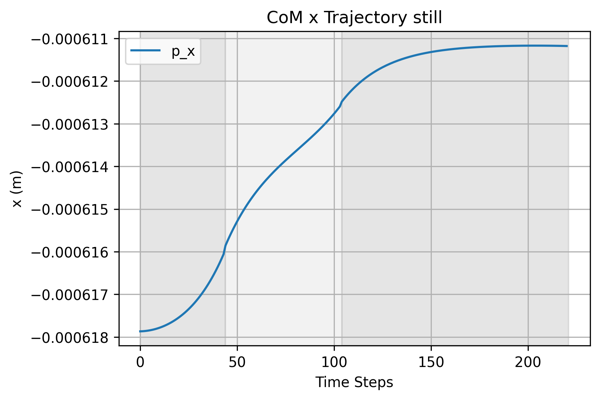
\includegraphics[width=\textwidth]{figures/CoM x Trajectory still.png}
        \caption{CoM x component}
        \label{fig:sub1}
    \end{subfigure}
    \hfill
    \begin{subfigure}[b]{0.32\textwidth}
        \centering
        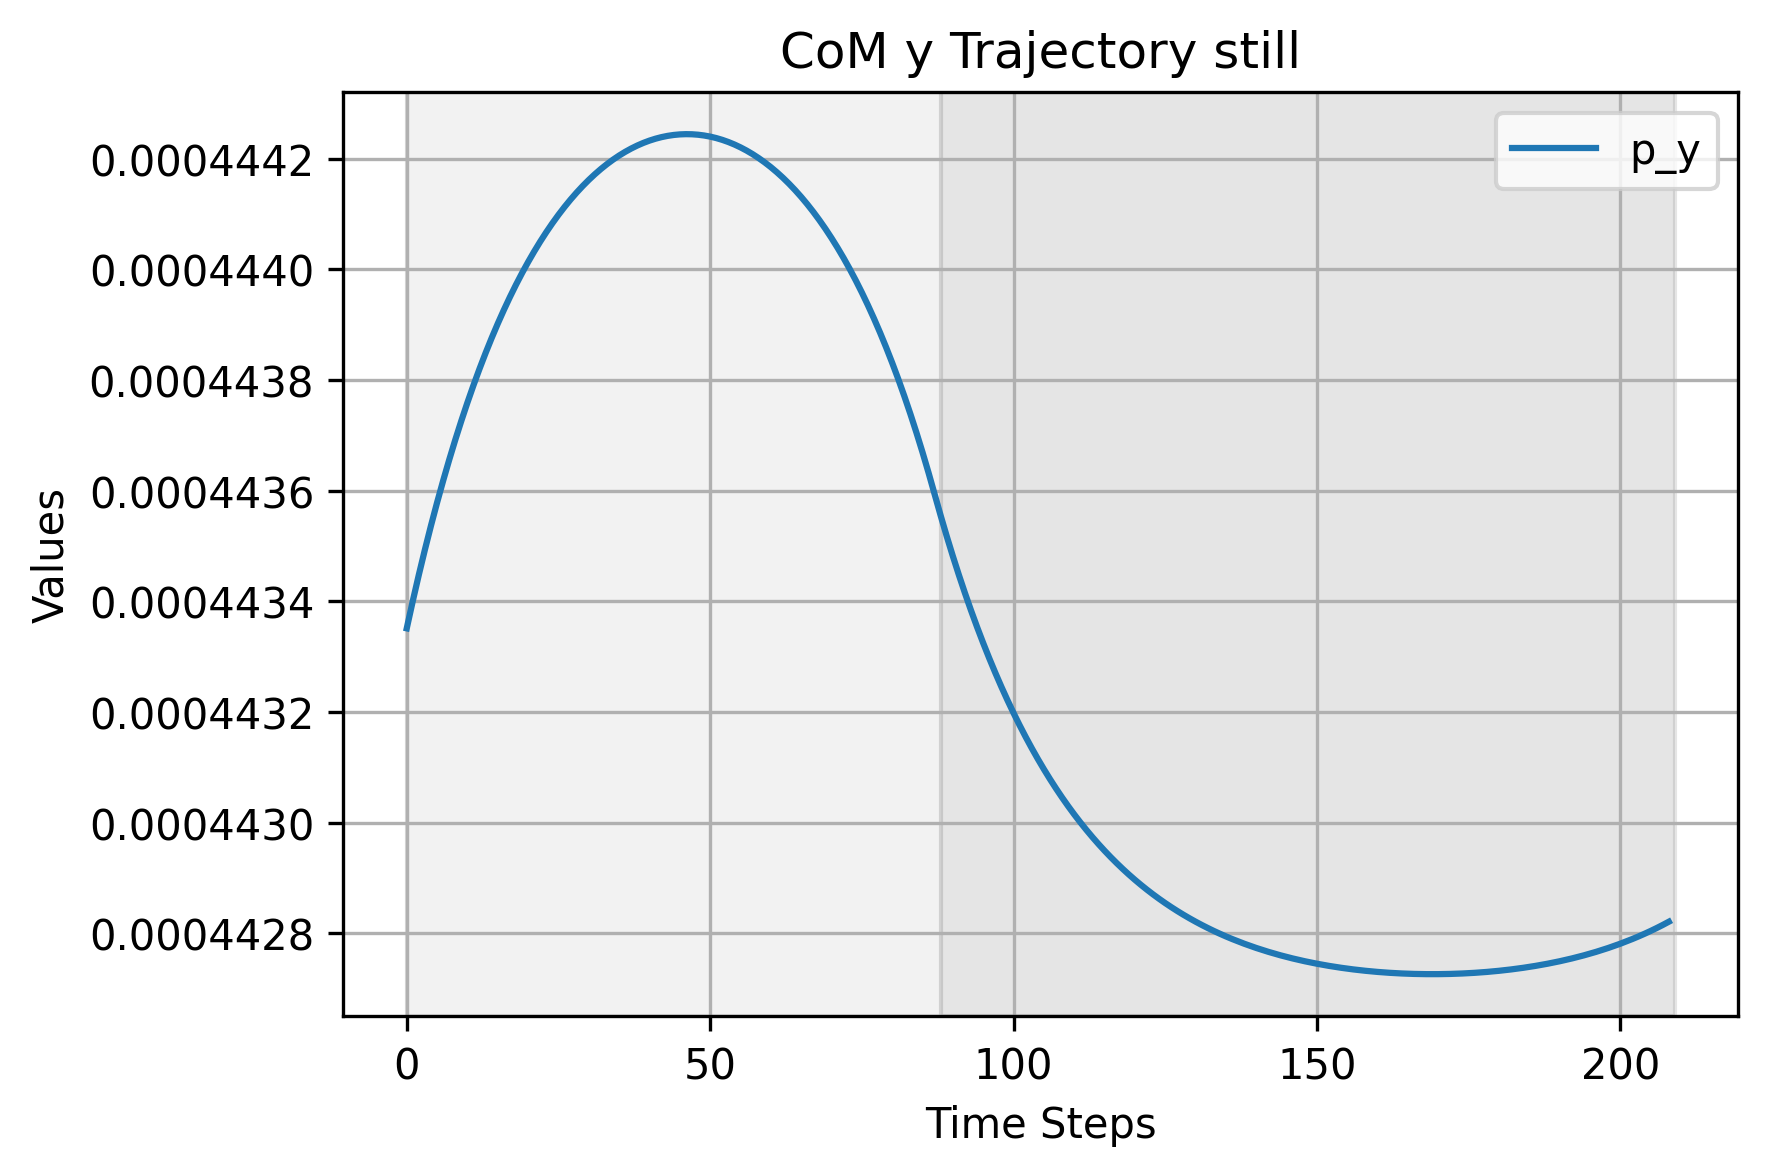
\includegraphics[width=\textwidth]{figures/CoM y Trajectory still.png}
        \caption{CoM y component}
        \label{fig:sub2}
    \end{subfigure}
    \hfill
    \begin{subfigure}[b]{0.32\textwidth}
        \centering
        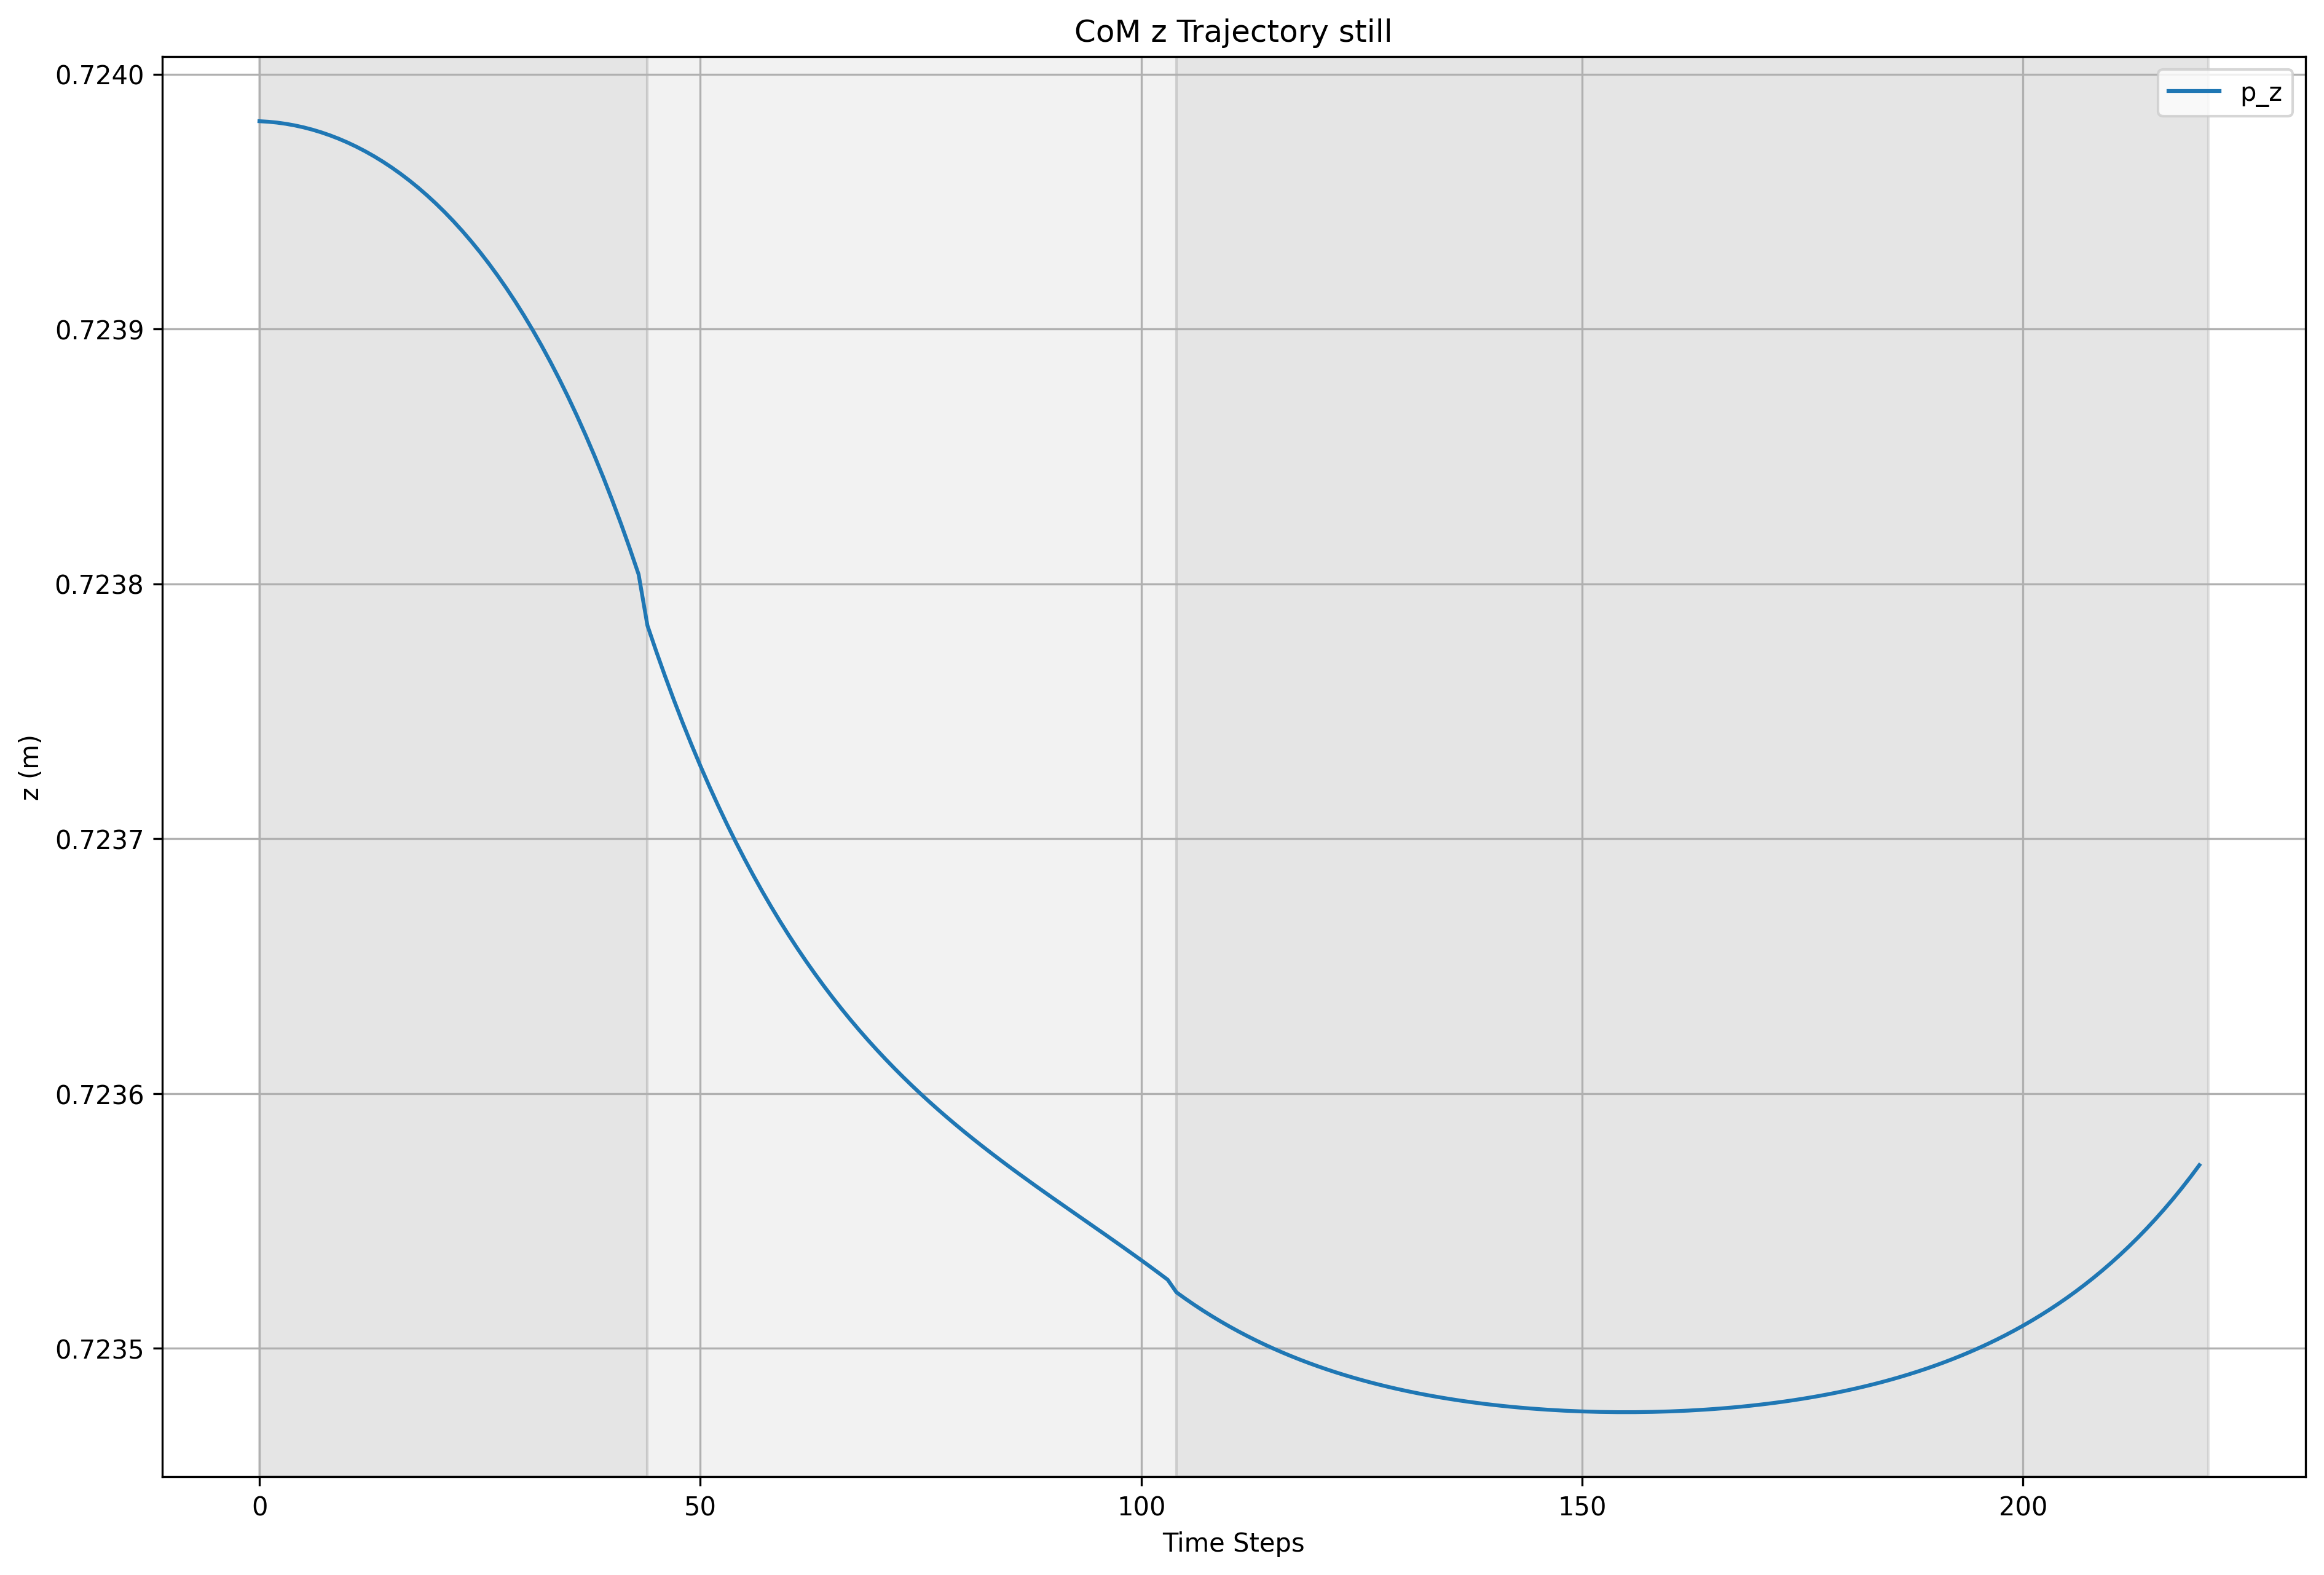
\includegraphics[width=\textwidth]{figures/CoM z Trajectory still.png}
        \caption{CoM z component}
        \label{fig:sub3}
    \end{subfigure}
    \caption{Evolution of CoM Position - Still Task}
    \label{fig:threeimages}
\end{figure}
In Figure 12, the evolution of the feet positions along the Z-axis, CoM velocity, and angular momentum during the still task is depicted. As expected for a stationary task, the Z-axis positions of both feet remain nearly constant, indicating that both feet maintain ground contact throughout the duration. The CoM velocity components (X, Y, Z) exhibit minimal variations, approaching zero as the system stabilizes, indicating effective maintenance of the stationary state. The angular momentum components (Lx, Ly, Lz) exhibit small fluctuations, suggesting slight corrective torques applied to maintain stability. These variations indicate the system’s capacity to counteract minor disturbances while achieving the desired stationary state. 
\begin{figure}[htbp]
    \centering
    \begin{subfigure}[b]{0.32\textwidth}
        \centering
        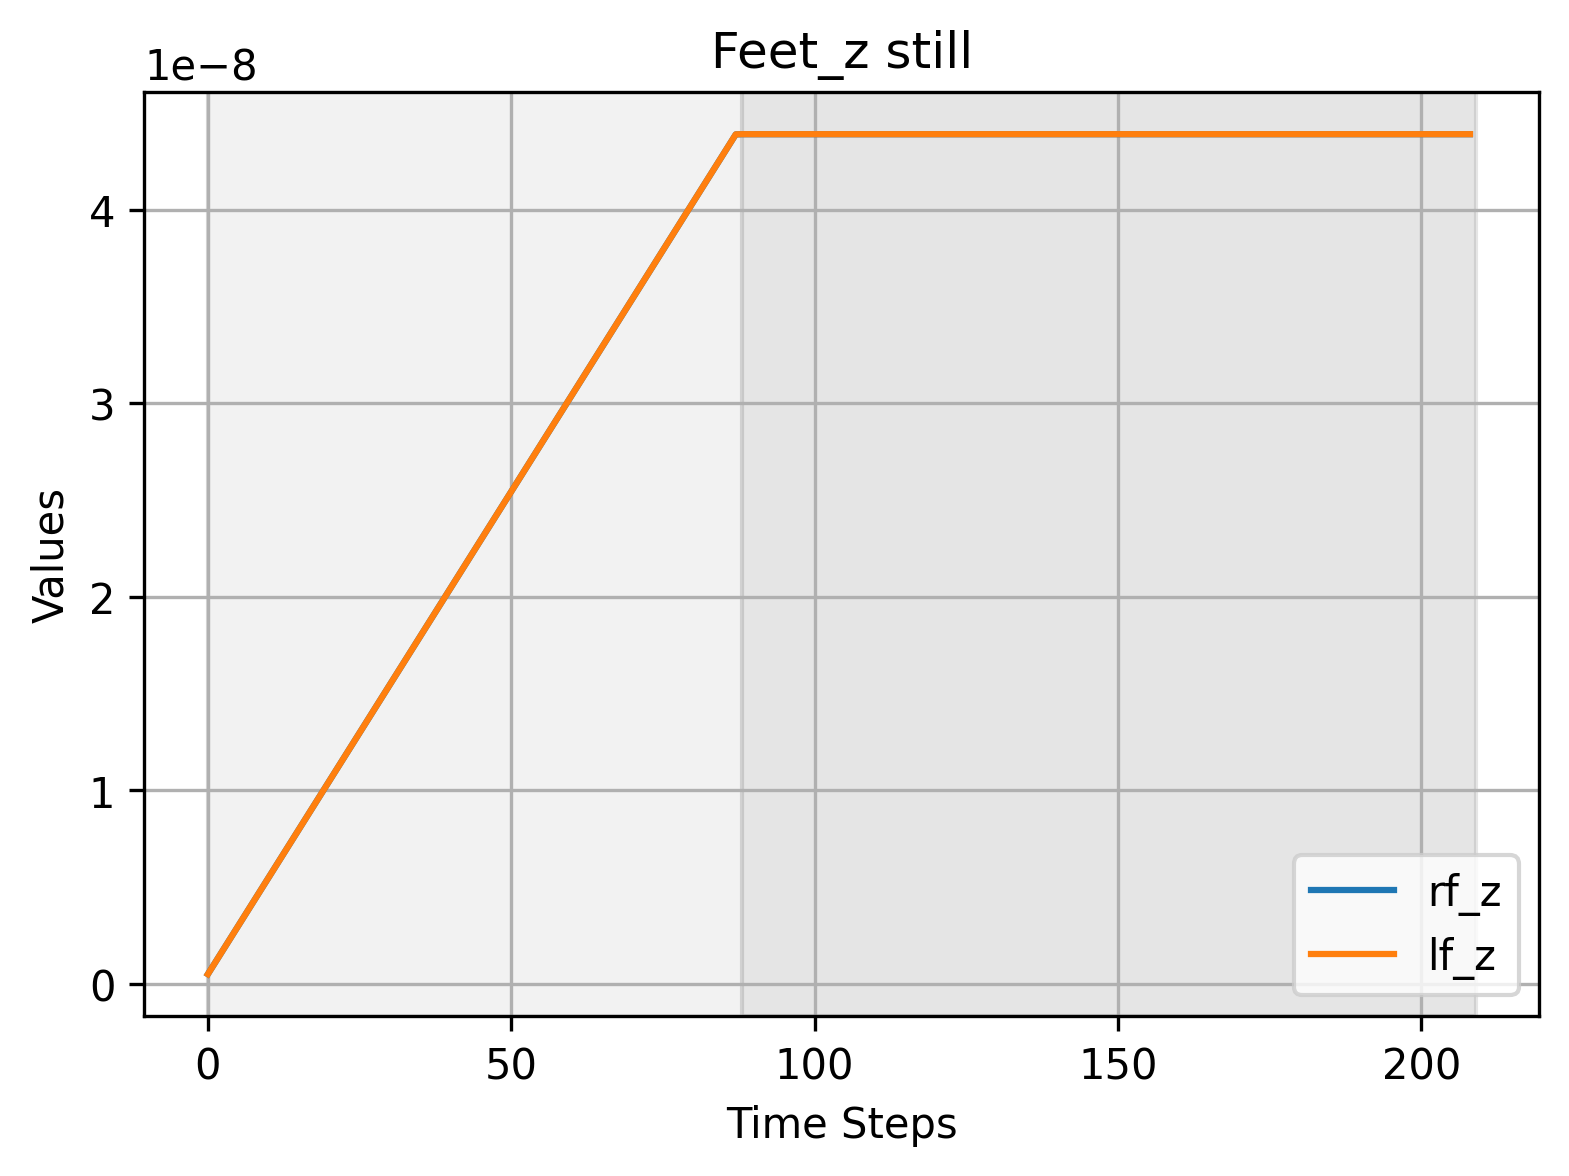
\includegraphics[width=\textwidth]{figures/Feet_z still.png}
        \caption{Feet along z axis}
        \label{fig:sub1}
    \end{subfigure}
    \hfill
    \begin{subfigure}[b]{0.32\textwidth}
        \centering
        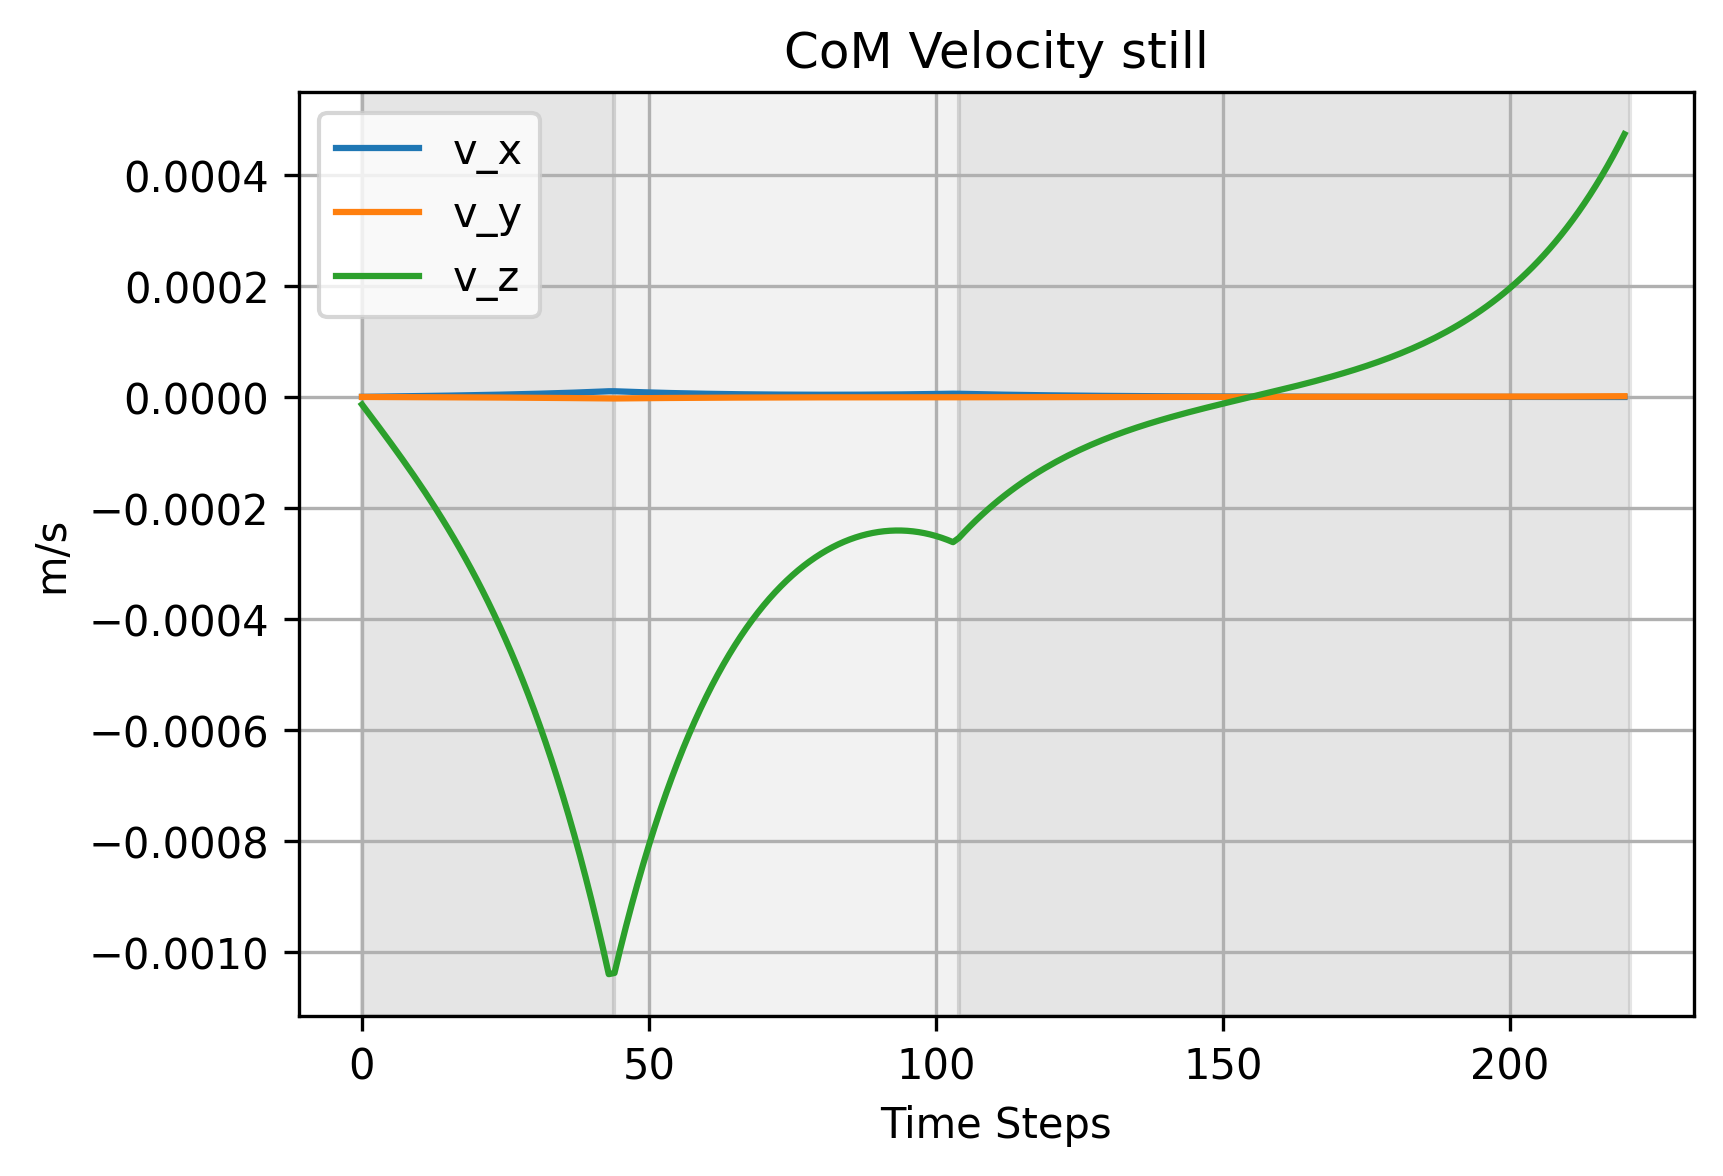
\includegraphics[width=\textwidth]{figures/CoM Velocity still.png}
        \caption{CoM Velocity}
        \label{fig:sub2}
    \end{subfigure}
    \hfill
    \begin{subfigure}[b]{0.32\textwidth}
        \centering
        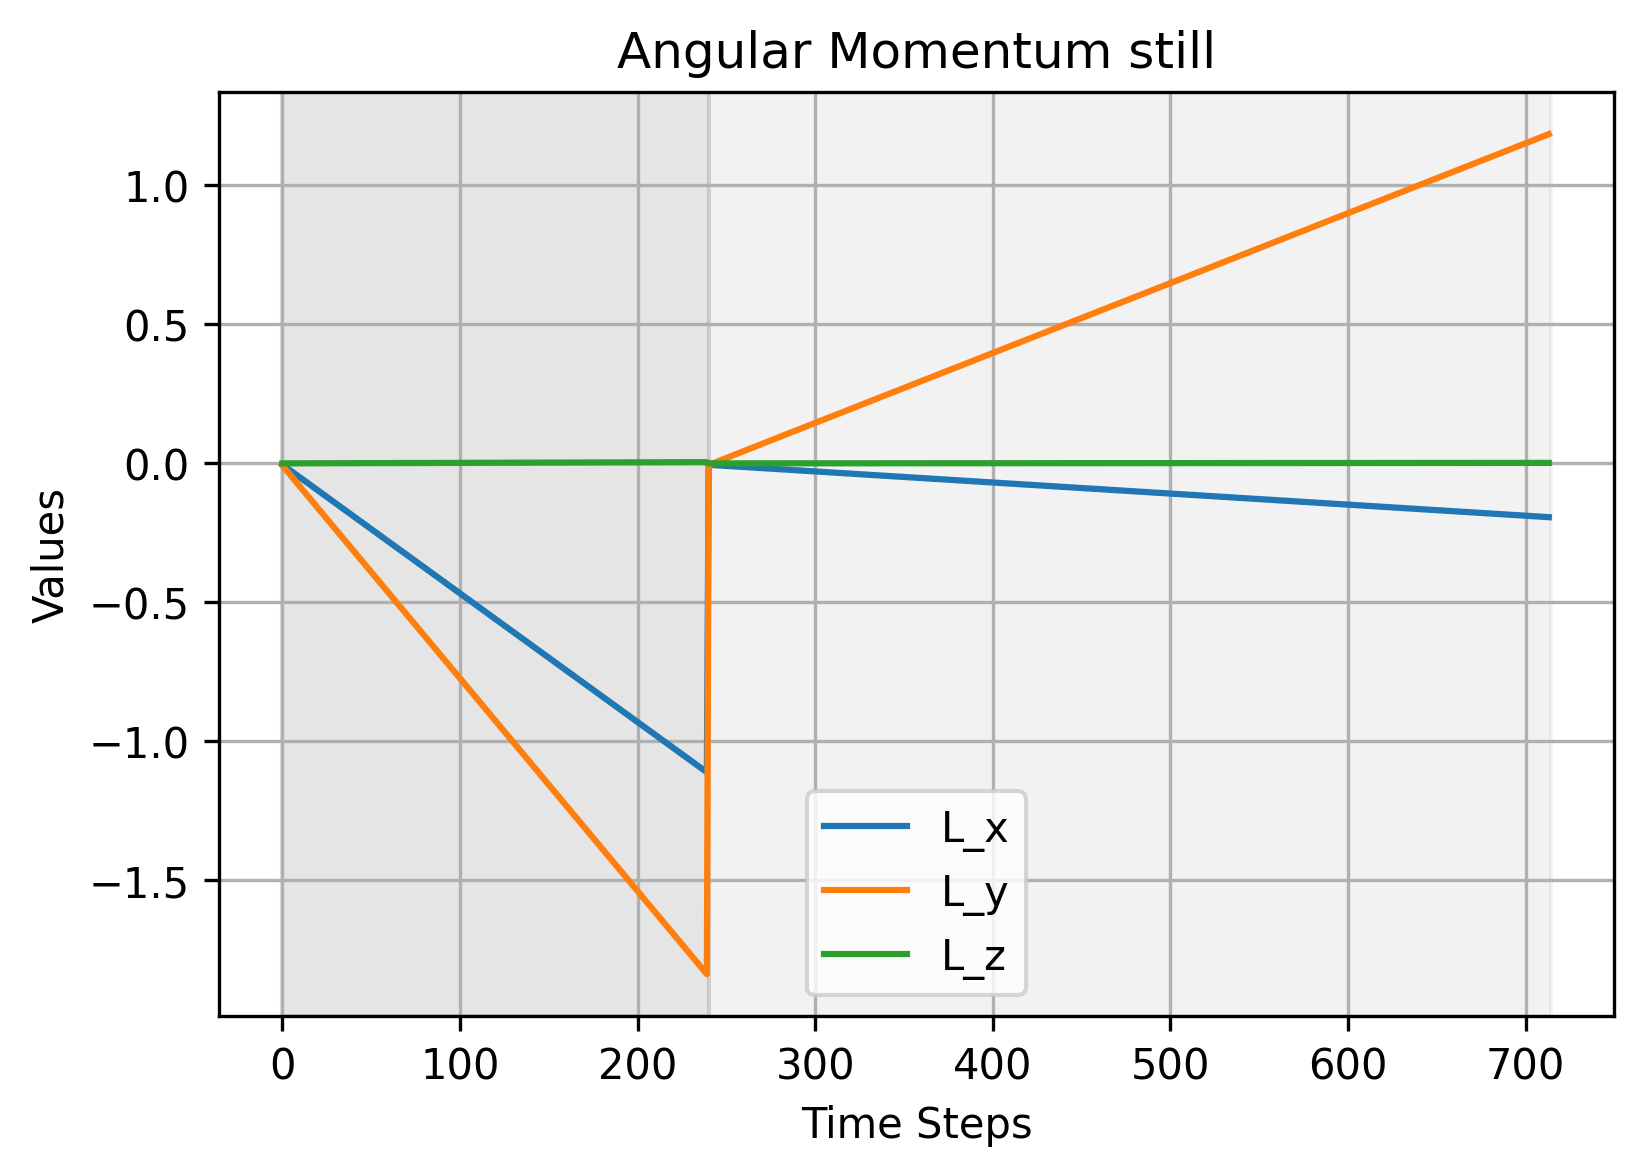
\includegraphics[width=\textwidth]{figures/Angular Momentum still.png}
        \caption{Angular Momentum}
        \label{fig:sub3}
    \end{subfigure}
    \caption{Feet, Com Velocity and Angular Momentum - Still Task}
    \label{fig:threeimages}
\end{figure}
In Figure 13, the comparison between the reference trajectory and the actual trajectory for the still task is presented. The CoM position components (X, Y, Z) remain relatively close to the reference, with minor deviations, particularly in the Y component, indicating small oscillations rather than perfect stillness.

The CoM velocity plots show slight fluctuations around zero, reflecting minor corrective adjustments, while the reference trajectory remains consistently flat. The angular momentum components exhibit noticeable deviations from the reference, especially in the X and Y directions, suggesting small but persistent torques being applied to maintain balance.

For the feet positions, both feet remain essentially stationary with minimal displacement, aligning well with the reference. The foot velocities confirm this, showing values close to zero, consistent with the intended stationary task.

Overall, the observed deviations highlight the system's attempts to maintain a stationary posture, though slight oscillations and corrective actions are present across multiple components.
\begin{figure}[htbp]
    \centering
    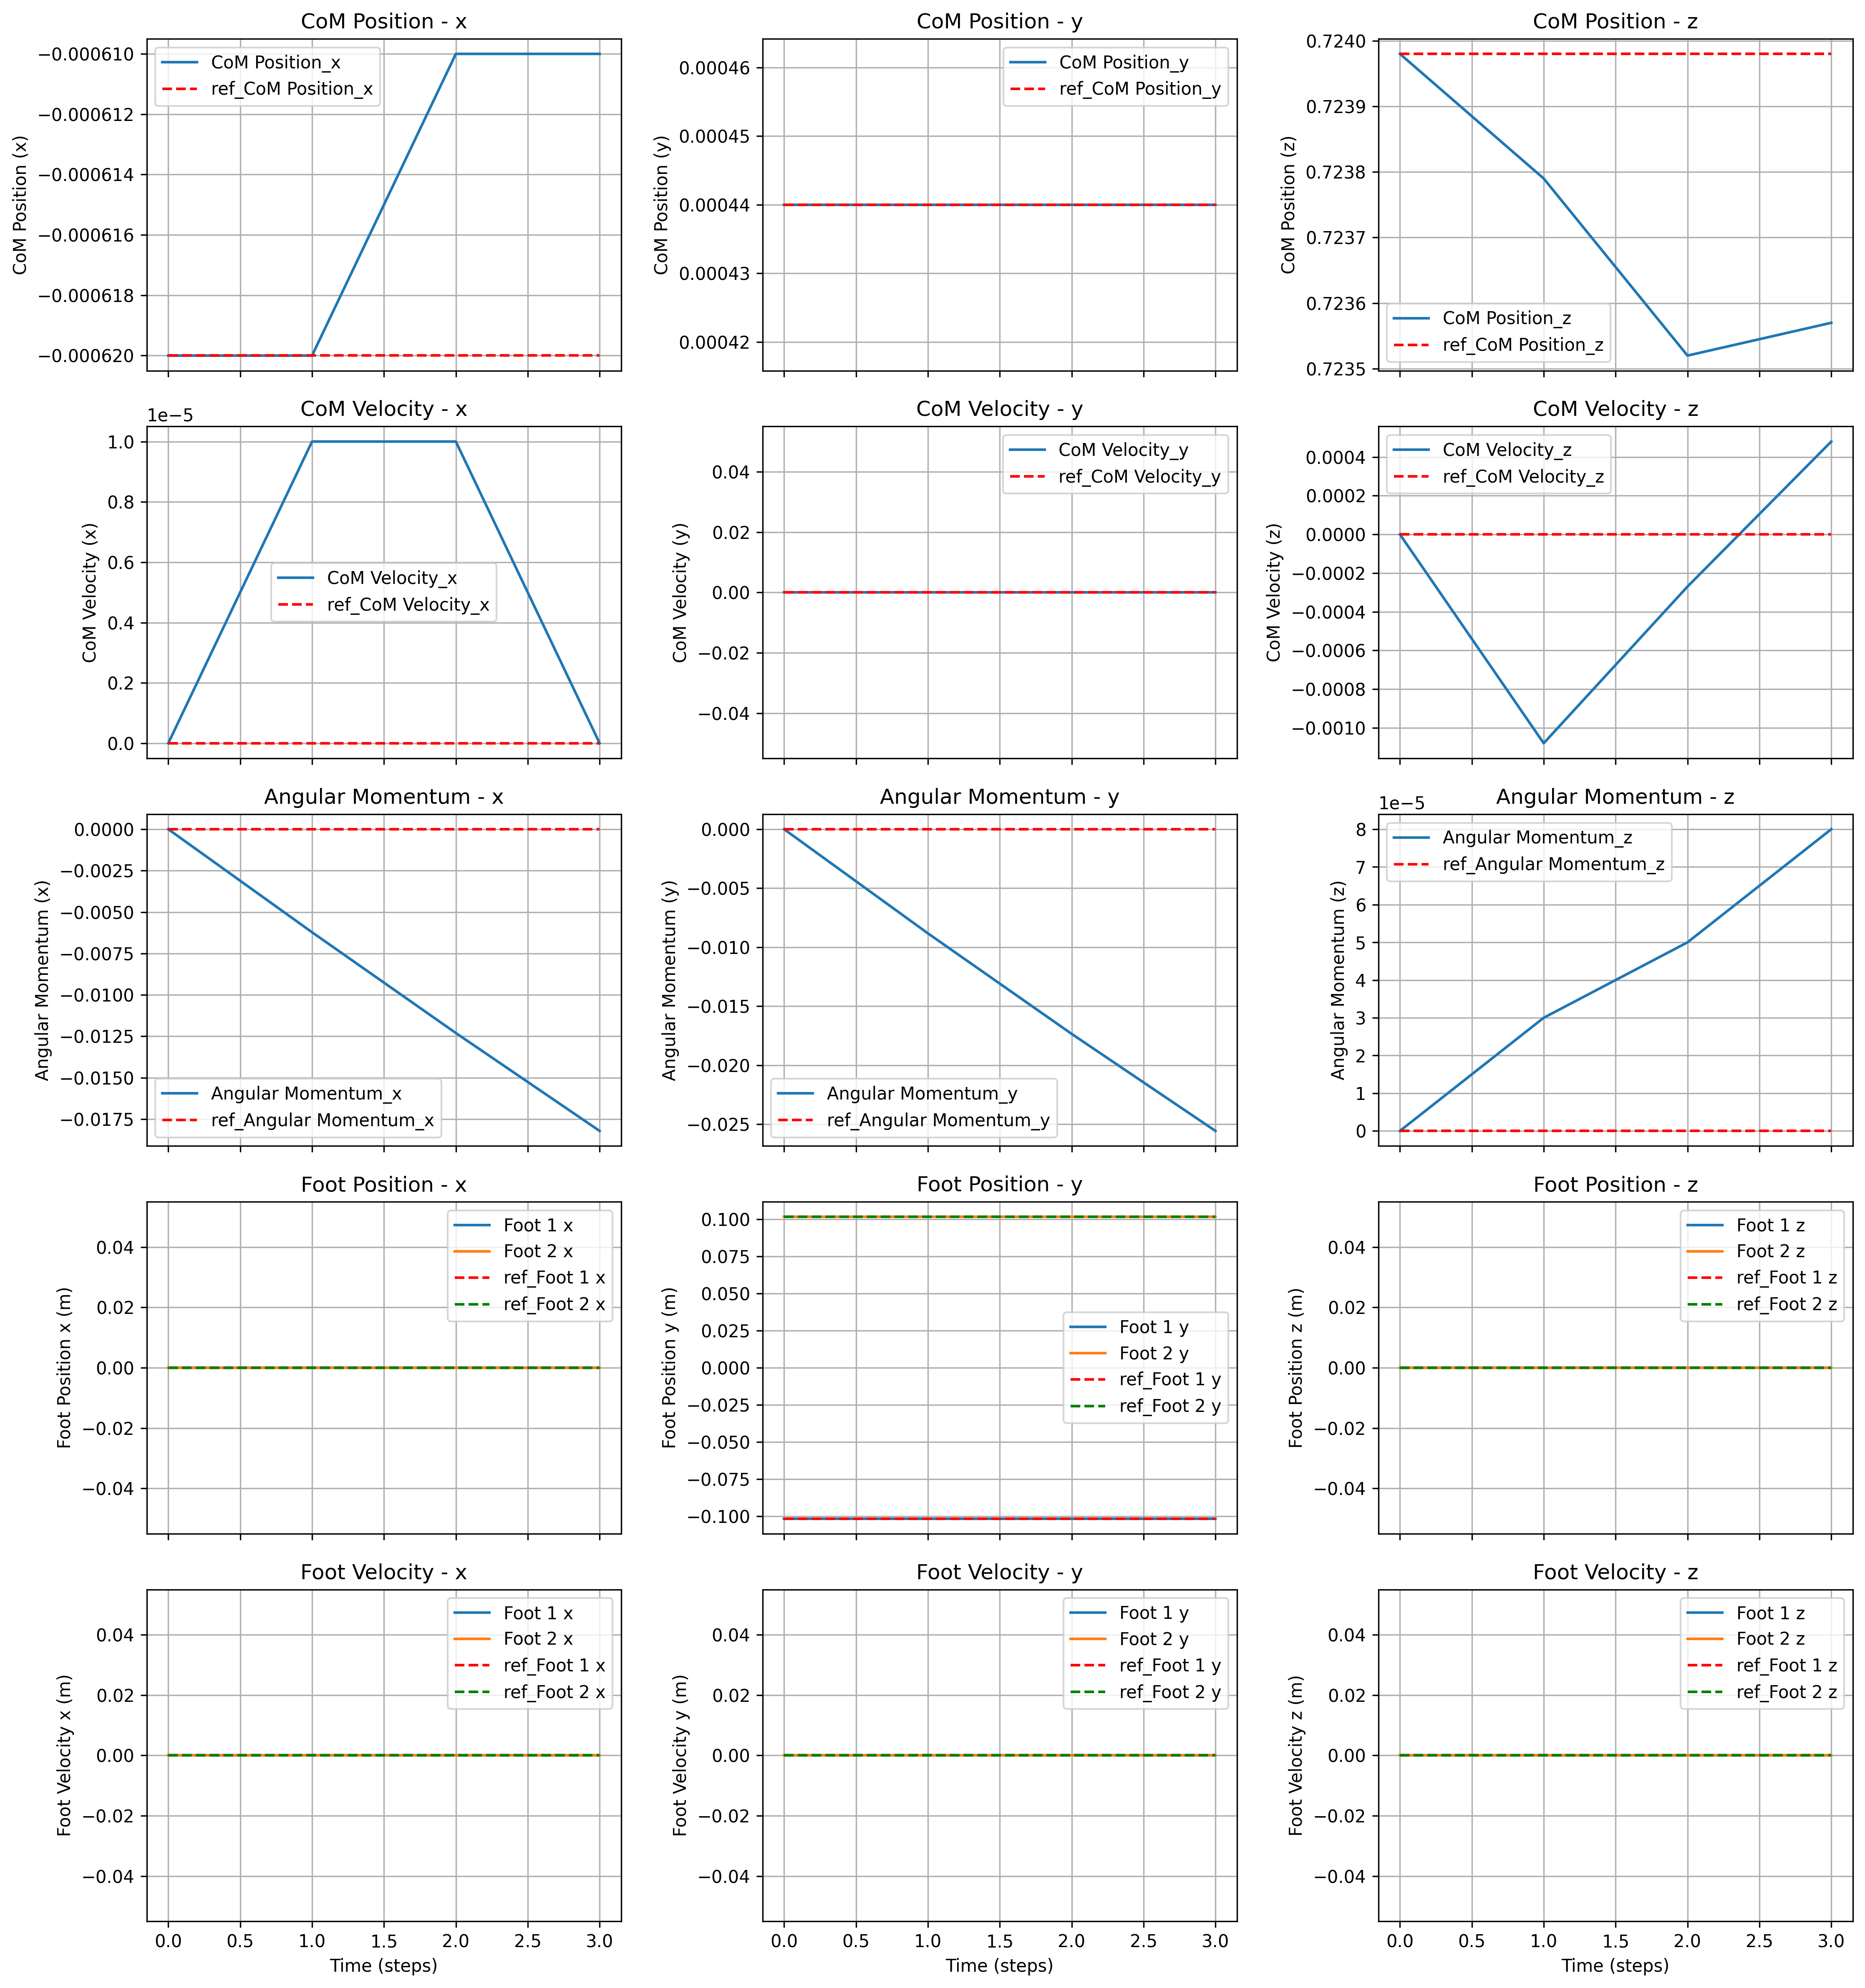
\includegraphics[width=0.8\textwidth]{figures/contact_x_still.png}
    \caption{Trajectory vs Reference - Still Task}
    \label{fig:yourlabel}
\end{figure}
\begin{table}[H]
    \centering
    \renewcommand{\arraystretch}{1.2}
    \resizebox{\textwidth}{!}{
        \begin{tabular}{c|c|c|c|c}
            \hline
            Interval & Right Foot (x,y,z) & Left Foot (x,y,z) & $\Sigma L_k$ & Sum Forces (x,y,z) \\
            \hline
            0 & (-0.0598, 10.005, 70.689) & (-0.0598, -9.920, 70.689) & (0, 0) & (-0.1196, 0.0855, 141.379) \\
            1 & (0.0002, 9.537, 48.988) & (0.0002, -9.537, 48.993) & (0, 0) & (0.0003, -0.0002, 97.980) \\
            2 & (-0.0002, 9.539, 49.085) & (-0.0001, -9.538, 49.090) & (0, 0) & (-0.0003, 0.0002, 98.174) \\
            \hline
        \end{tabular}
    }
    \caption{Summary of Forces and Foot Positions per Interval - Still Task}
    \label{tab:data_table}
\end{table}
In Figure 14, the comparison between the reference forces and the generated forces for the still task is presented. The translational forces (F\_x, F\_y, F\_z) exhibit periodic oscillations, deviating slightly from the reference, particularly in the Z component, where larger fluctuations are observed. These deviations indicate minor adjustments to maintain stability while compensating for small disturbances.
The rotational forces (ETA\_x, ETA\_y, ETA\_z) similarly display oscillatory patterns, with noticeable variations from the reference, suggesting corrective actions to counteract small perturbations. The overall trend shows a recurring pattern, indicating that despite the still task objective, the system is actively modulating forces to maintain balance.
\begin{figure}[htbp]
    \centering
    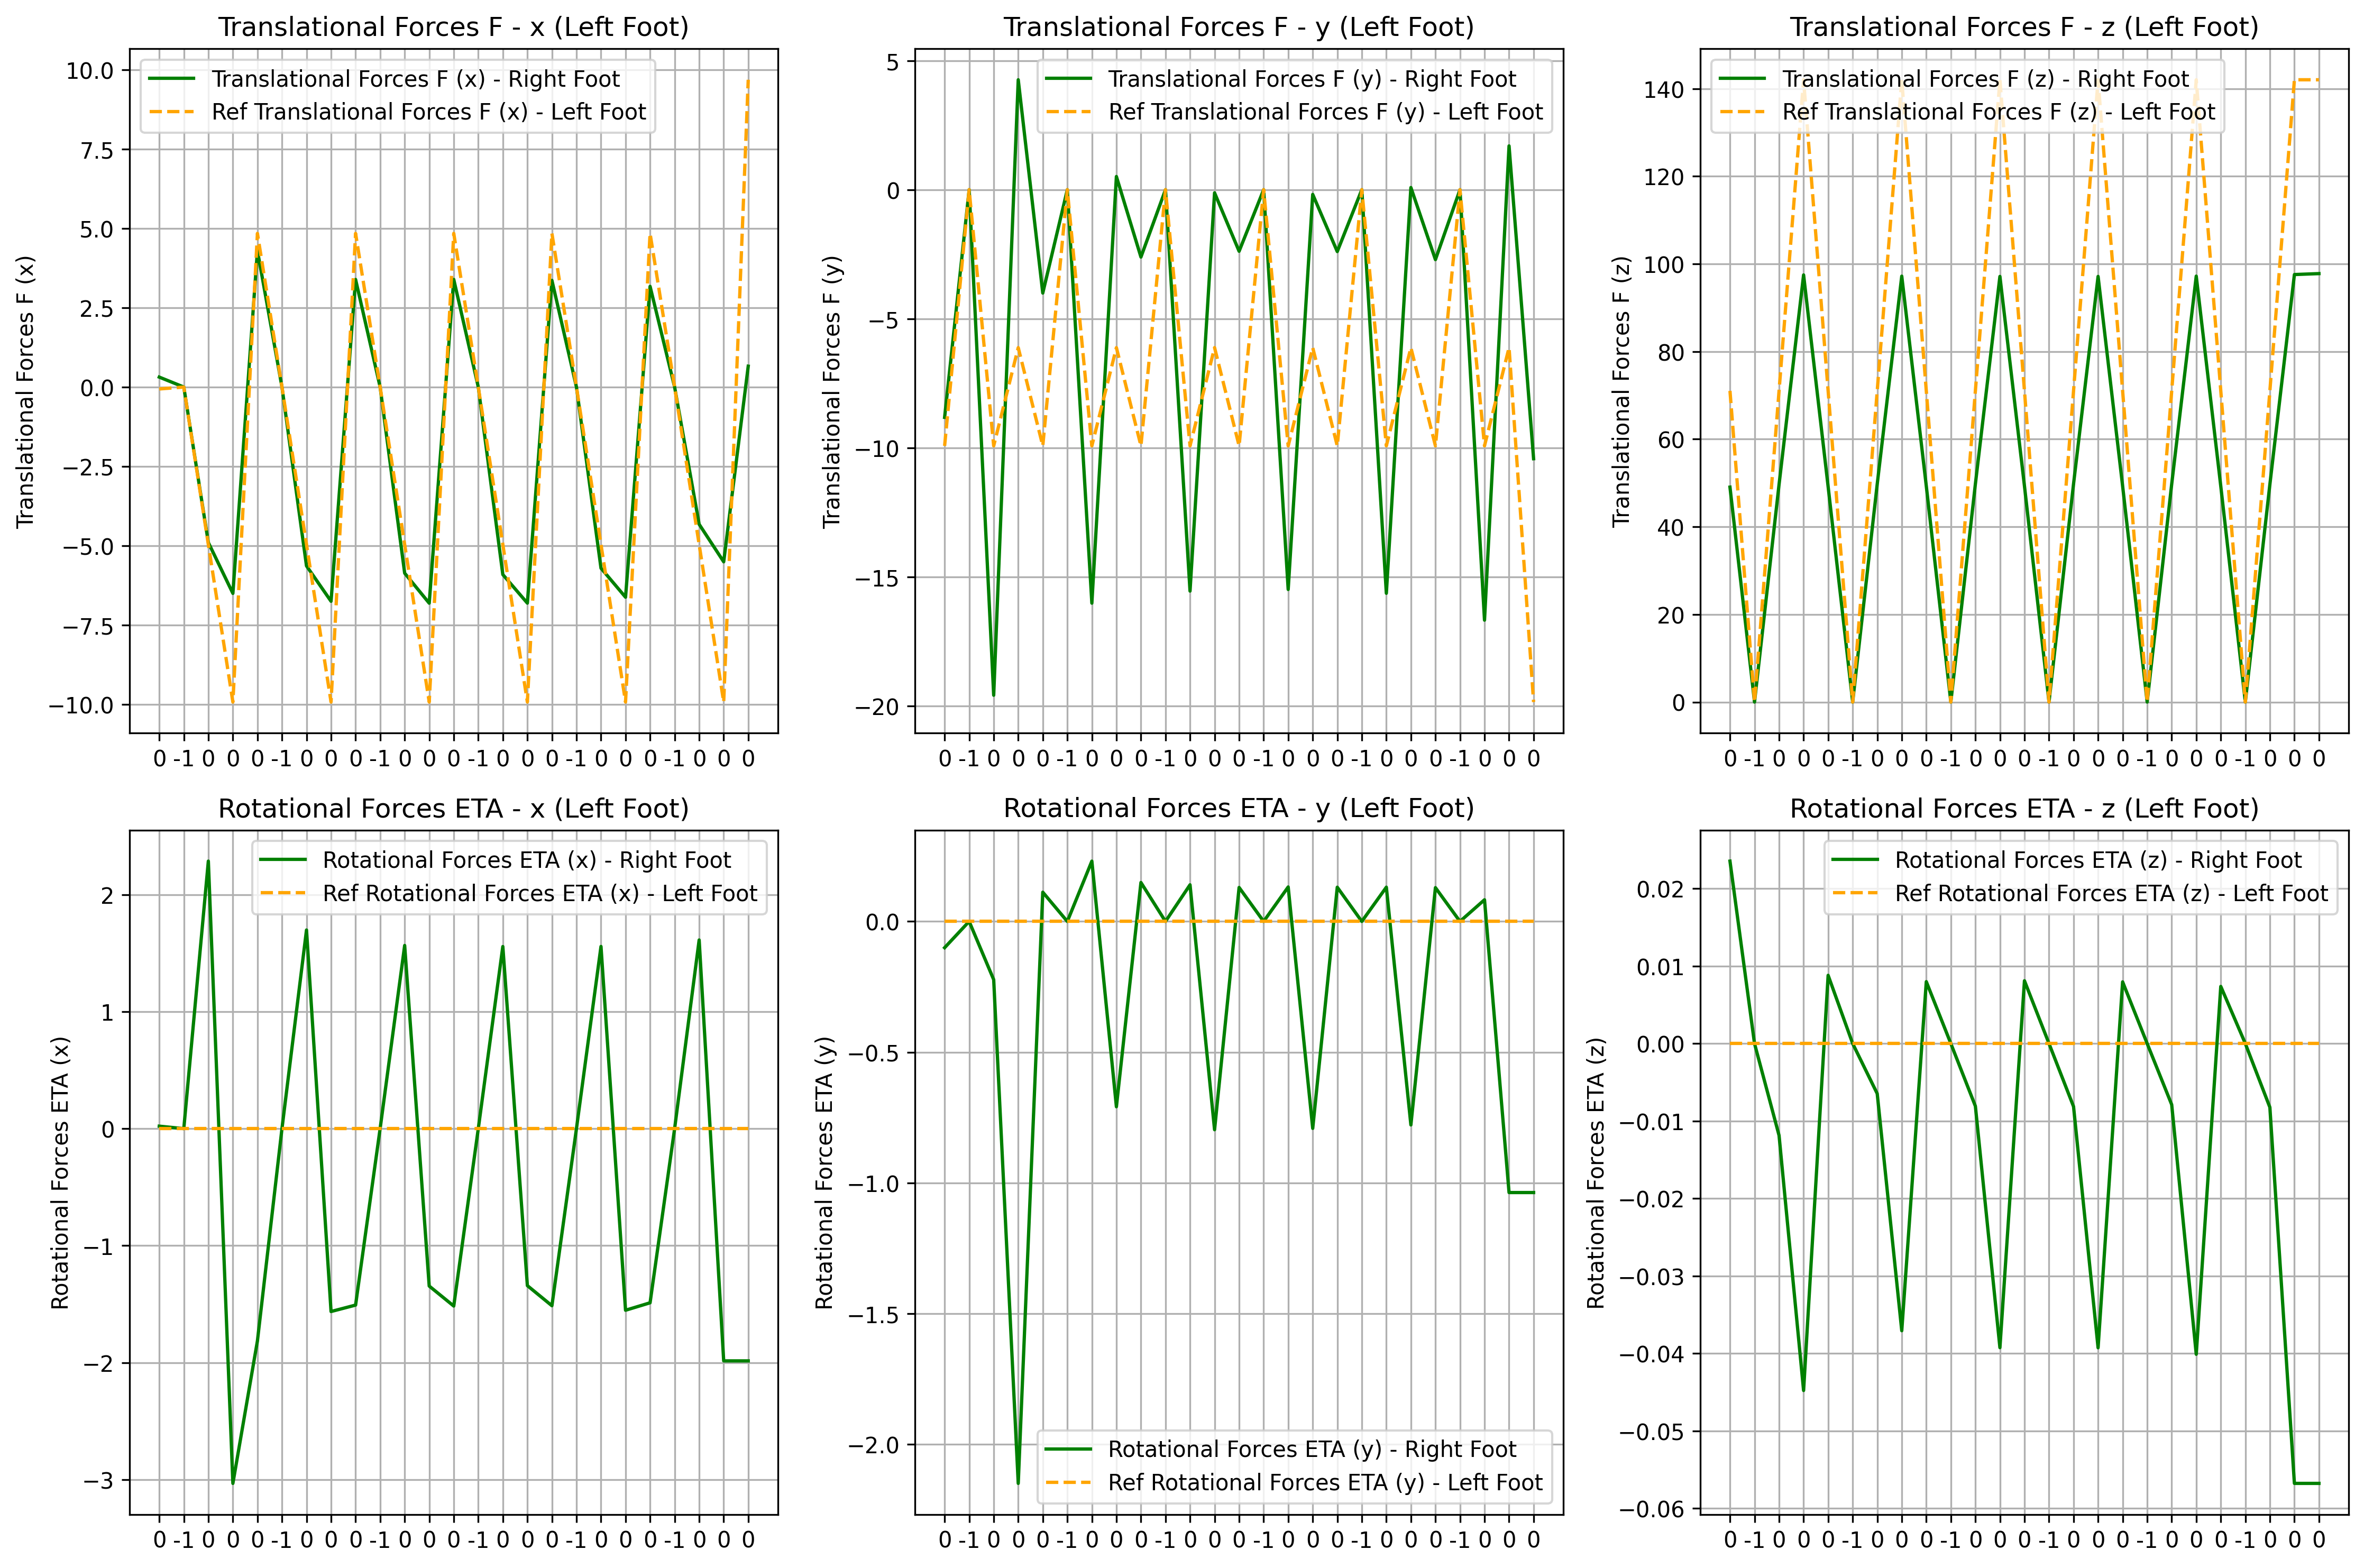
\includegraphics[width=0.8\textwidth]{figures/contact_forces_walking.png}
    \caption{Trajectory vs Reference Forces - Still Task}
    \label{fig:contact_forces_walking}
\end{figure}

%\paragraph{}   
\subsection{Walking Task}
Generalities about the walking task. 
\paragraph{Reference Trajectory Generation}
In the walking task, the trajectory is designed to simulate a natural walking pattern by coordinating the movements of the feet and the Center of Mass (CoM) through a sequence of double-support and single-support phases. During double-support phases, when both feet are in contact with the ground, the CoM remains stationary, providing stability. Movement along the X-axis occurs only during single-support phases, where one foot is lifted and the other remains grounded.

The CoM position update depends on the preceding phase. If the previous phase was double-support, the CoM remains at its current position. However, if the previous phase was single-support, the CoM advances by a specified displacement, ensuring consistent forward movement and balance.

The foot trajectory is constructed to simulate a natural step, where the foot in motion extends beyond the stationary foot. The Z-coordinate of each foot is set to zero at the start of each phase, representing ground contact. As the foot moves during the single-support phase, its height follows a parabolic profile, allowing for a smooth lift-off and descent. This profile is determined by interpolating between the start and end positions defined by the phase solutions, ensuring continuity and preventing abrupt changes.

Furthermore, the X-coordinate of the moving foot is updated alternately, depending on which foot was lifted in the previous phase. This alternating pattern maintains rhythmic progression, effectively mimicking a natural walking cycle. Consequently, the contact sequence, as presented in Table 2, defines the specific sequence of double-support and single-support phases, guiding the transitions and timing of each step.

\begin{table}[h!]
    \label{tab:stilltask}
    \centering
    \begin{tabular}{|c|c|c|c|}
        \hline
        Task & N & Foot & Contact Sequence \\
        \hline
        Walk & 24 & Right & 000-000-000-000-000-0 \\
        & & Left & 0-000-000-000-000-000 \\
        \hline
    \end{tabular}
    \caption{Contact sequence for still task with foot column}
\end{table}

\paragraph{Simulation Results}
Say something about the walking task and the results here. \\ 
In Figure 15, the evolution of the CoM position components (X, Y, Z) during the walking task is illustrated. The X component shows a consistent upward trend, representing the forward progression of the CoM as the robot advances step by step. This steady increase is expected, as the walking task involves continuous forward movement. \\
The Y component exhibits a pronounced oscillatory pattern, corresponding to the lateral sway that naturally occurs as the robot shifts its weight from one foot to the other during each step. The regularity of these oscillations reflects the cyclic nature of the walking gait, with each peak and trough aligning with foot contact transitions. \\
The Z component also follows a periodic oscillation, capturing the vertical motion as the feet alternate between ground contact and lift-off. The amplitude of these oscillations is relatively small, indicating that the CoM height remains fairly stable, with slight variations caused by the foot lift and placement during each step.
\begin{figure}[H]
    \centering
    \begin{subfigure}[b]{0.32\textwidth}
        \centering
        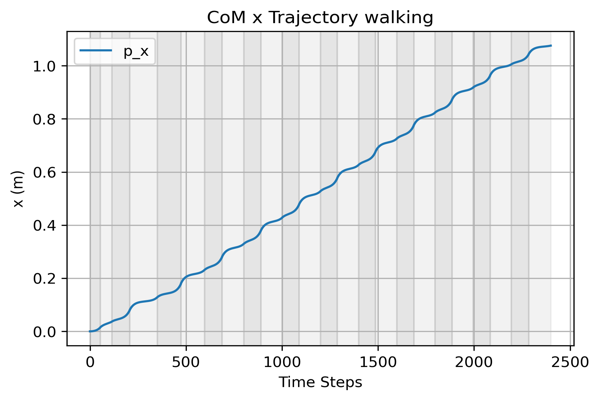
\includegraphics[width=\textwidth]{figures/CoM x Trajectory walking.png}
        \caption{CoM x component}
        \label{fig:sub1}
    \end{subfigure}
    \hfill
    \begin{subfigure}[b]{0.32\textwidth}
        \centering
        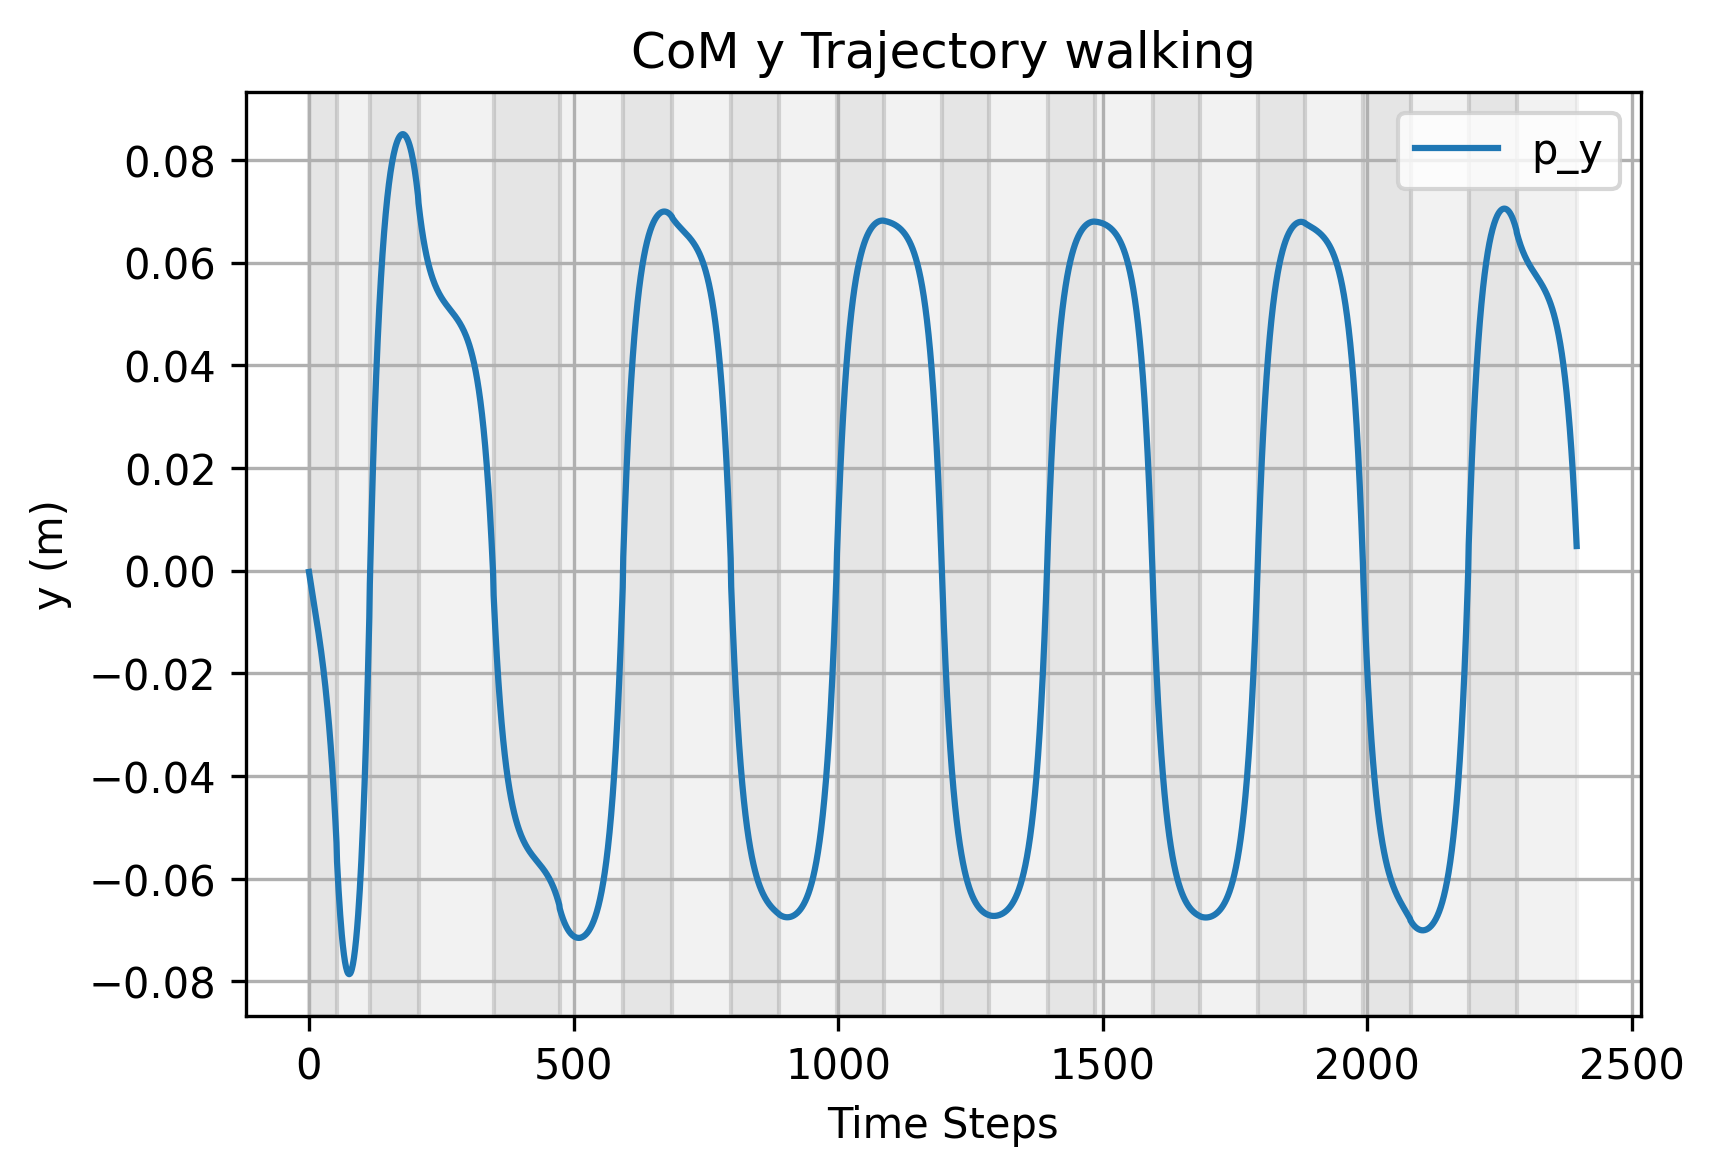
\includegraphics[width=\textwidth]{figures/CoM y Trajectory walking.png}
        \caption{CoM y component}
        \label{fig:sub2}
    \end{subfigure}
    \hfill
    \begin{subfigure}[b]{0.32\textwidth}
        \centering
        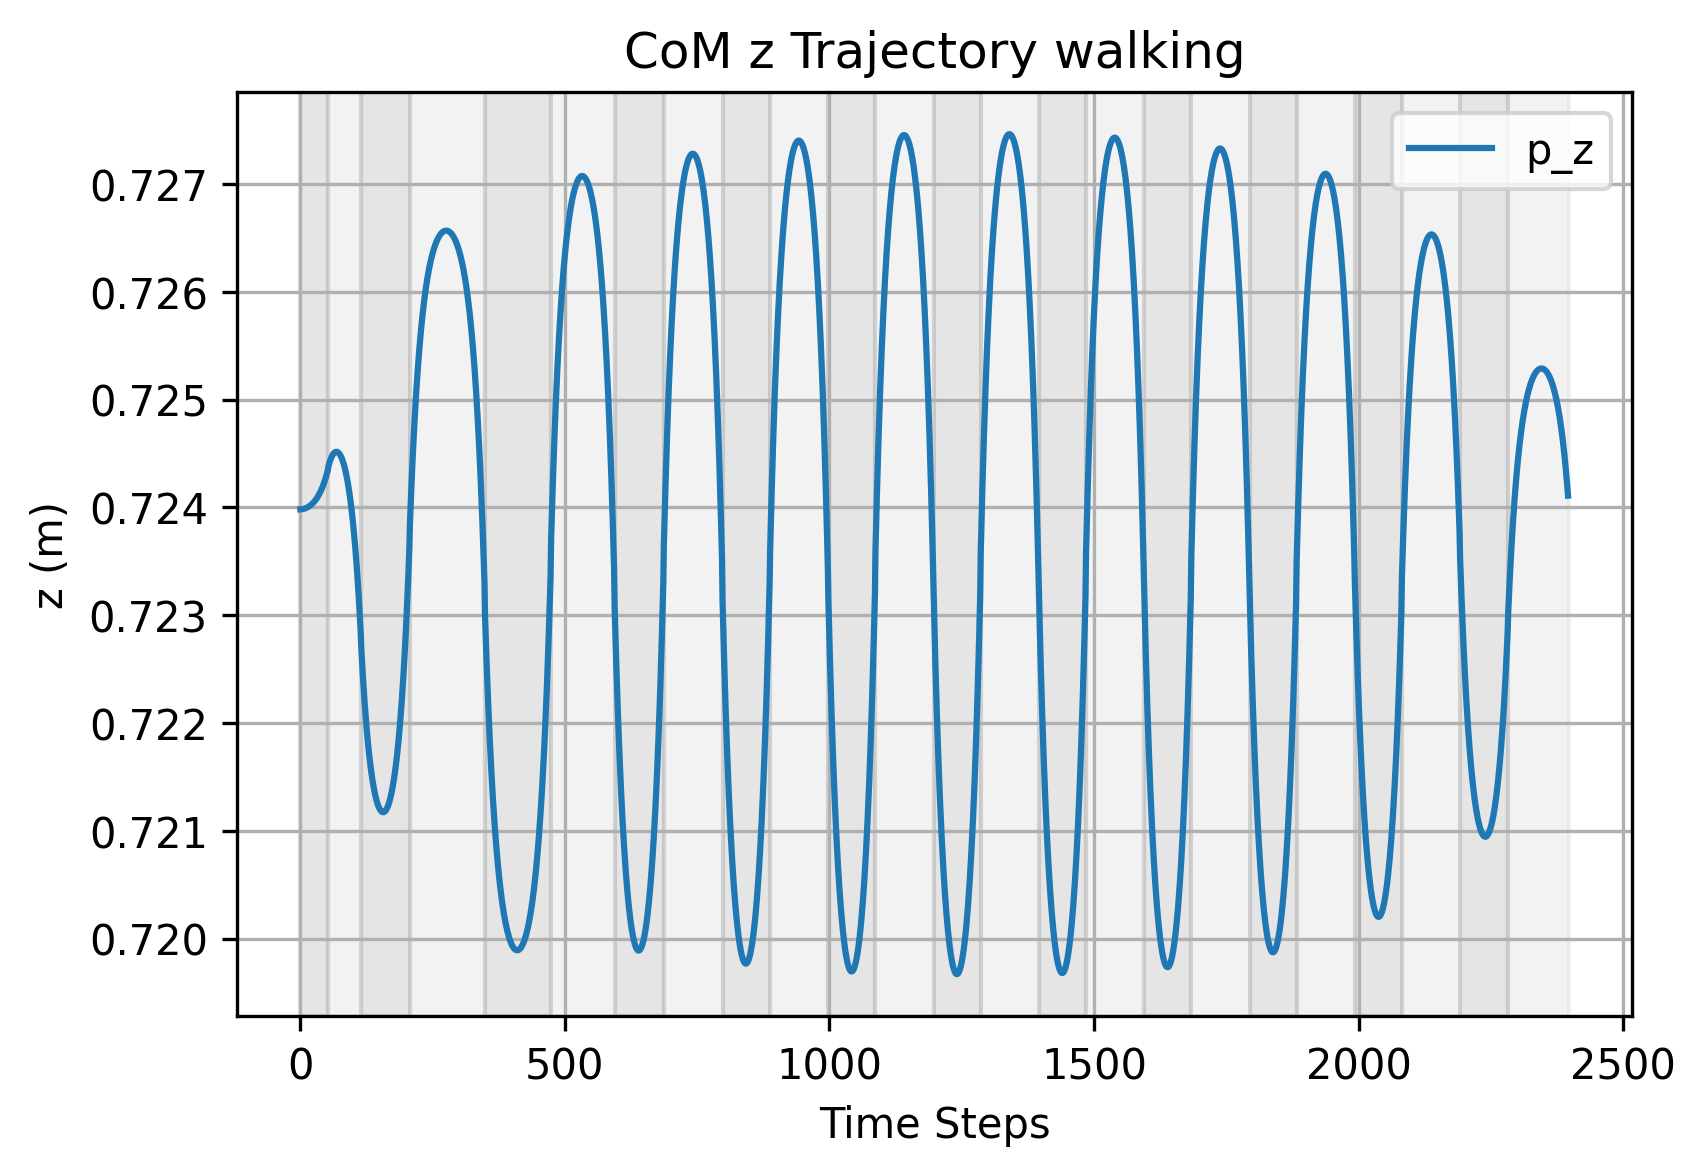
\includegraphics[width=\textwidth]{figures/CoM z Trajectory walking.png}
        \caption{CoM z component}
        \label{fig:sub3}
    \end{subfigure}
    \caption{Evolution of CoM Position - Walking Task}
    \label{fig:threeimages}
\end{figure}
In Figure 16, the evolution of the feet positions along the Z-axis, CoM velocity, and angular momentum during the walking task is presented.\\
The Z-axis foot positions exhibit periodic oscillations, representing the alternating lift-off and ground contact of each foot as the robot progresses through the walking gait. The regular pattern confirms the cyclic nature of the stepping sequence, with each peak corresponding to a foot being lifted and each trough indicating ground contact.\\
The CoM velocity components display distinct oscillatory patterns, with pronounced fluctuations in the X direction due to forward movement and periodic variations in the Y and Z components corresponding to lateral and vertical adjustments during each step. The consistent oscillations align with the alternating support phases and reflect the dynamic nature of walking.\\
The angular momentum components (Lx, Ly, Lz) show noticeable oscillations, particularly in the X component, indicating significant torques generated during each step to maintain balance and control. The cyclic nature of these oscillations is consistent with the alternating foot contact, highlighting the system’s continuous adjustments to maintain stability throughout the walking cycle.
\begin{figure}[htbp]
    \centering
    \begin{subfigure}[b]{0.32\textwidth}
        \centering
        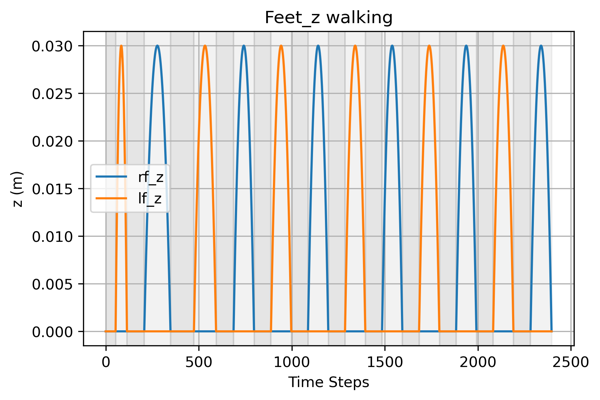
\includegraphics[width=\textwidth]{figures/Feet_z walking.png}
        \caption{Feet along z axis}
        \label{fig:sub1}
    \end{subfigure}
    \hfill
    \begin{subfigure}[b]{0.32\textwidth}
        \centering
        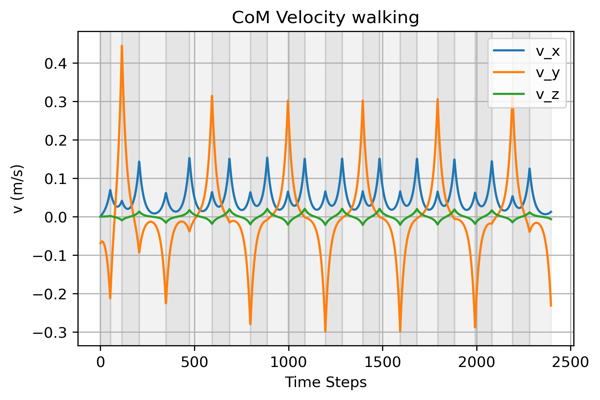
\includegraphics[width=\textwidth]{figures/CoM Velocity walking.png}
        \caption{CoM Velocity}
        \label{fig:sub2}
    \end{subfigure}
    \hfill
    \begin{subfigure}[b]{0.32\textwidth}
        \centering
        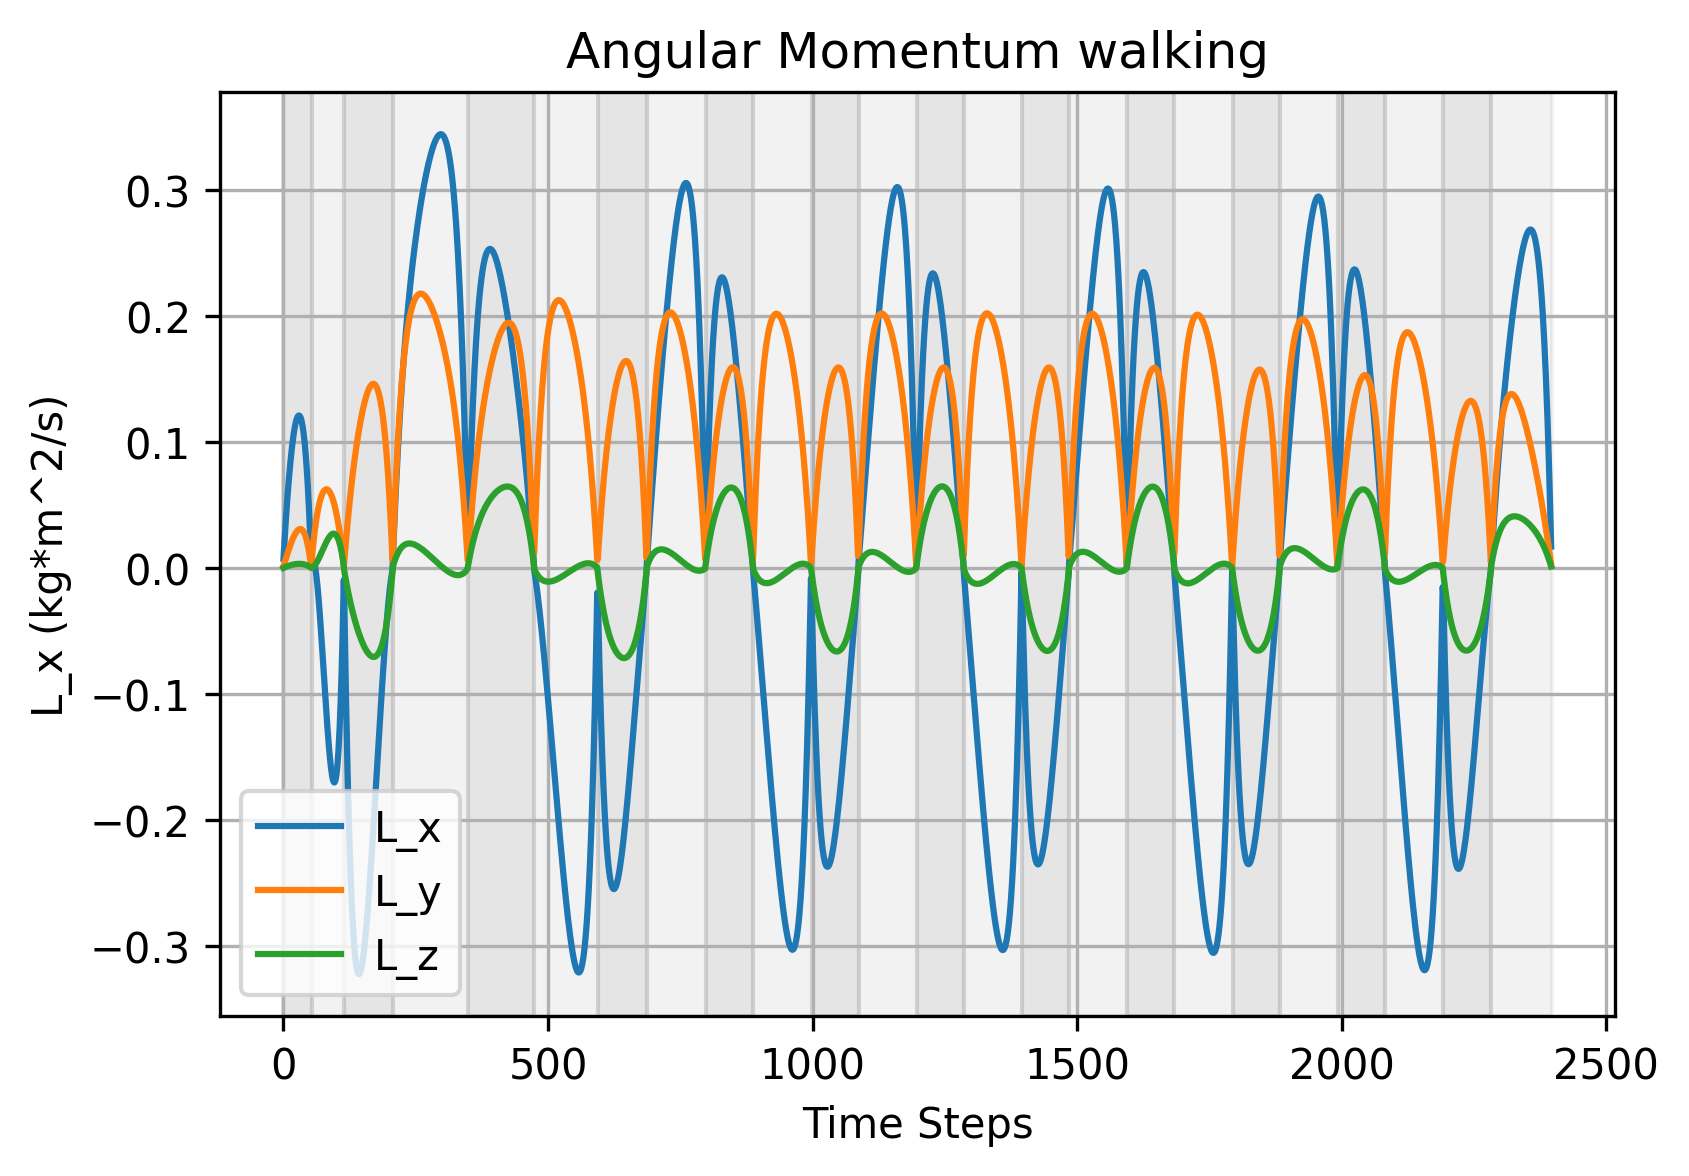
\includegraphics[width=\textwidth]{figures/Angular Momentum walking.png}
        \caption{Angular Momentum}
        \label{fig:sub3}
    \end{subfigure}
    \caption{Feet, Com Velocity and Angular Momentum - Walking Task}
    \label{fig:threeimages}
\end{figure}
\begin{figure}[htbp]
    \centering
    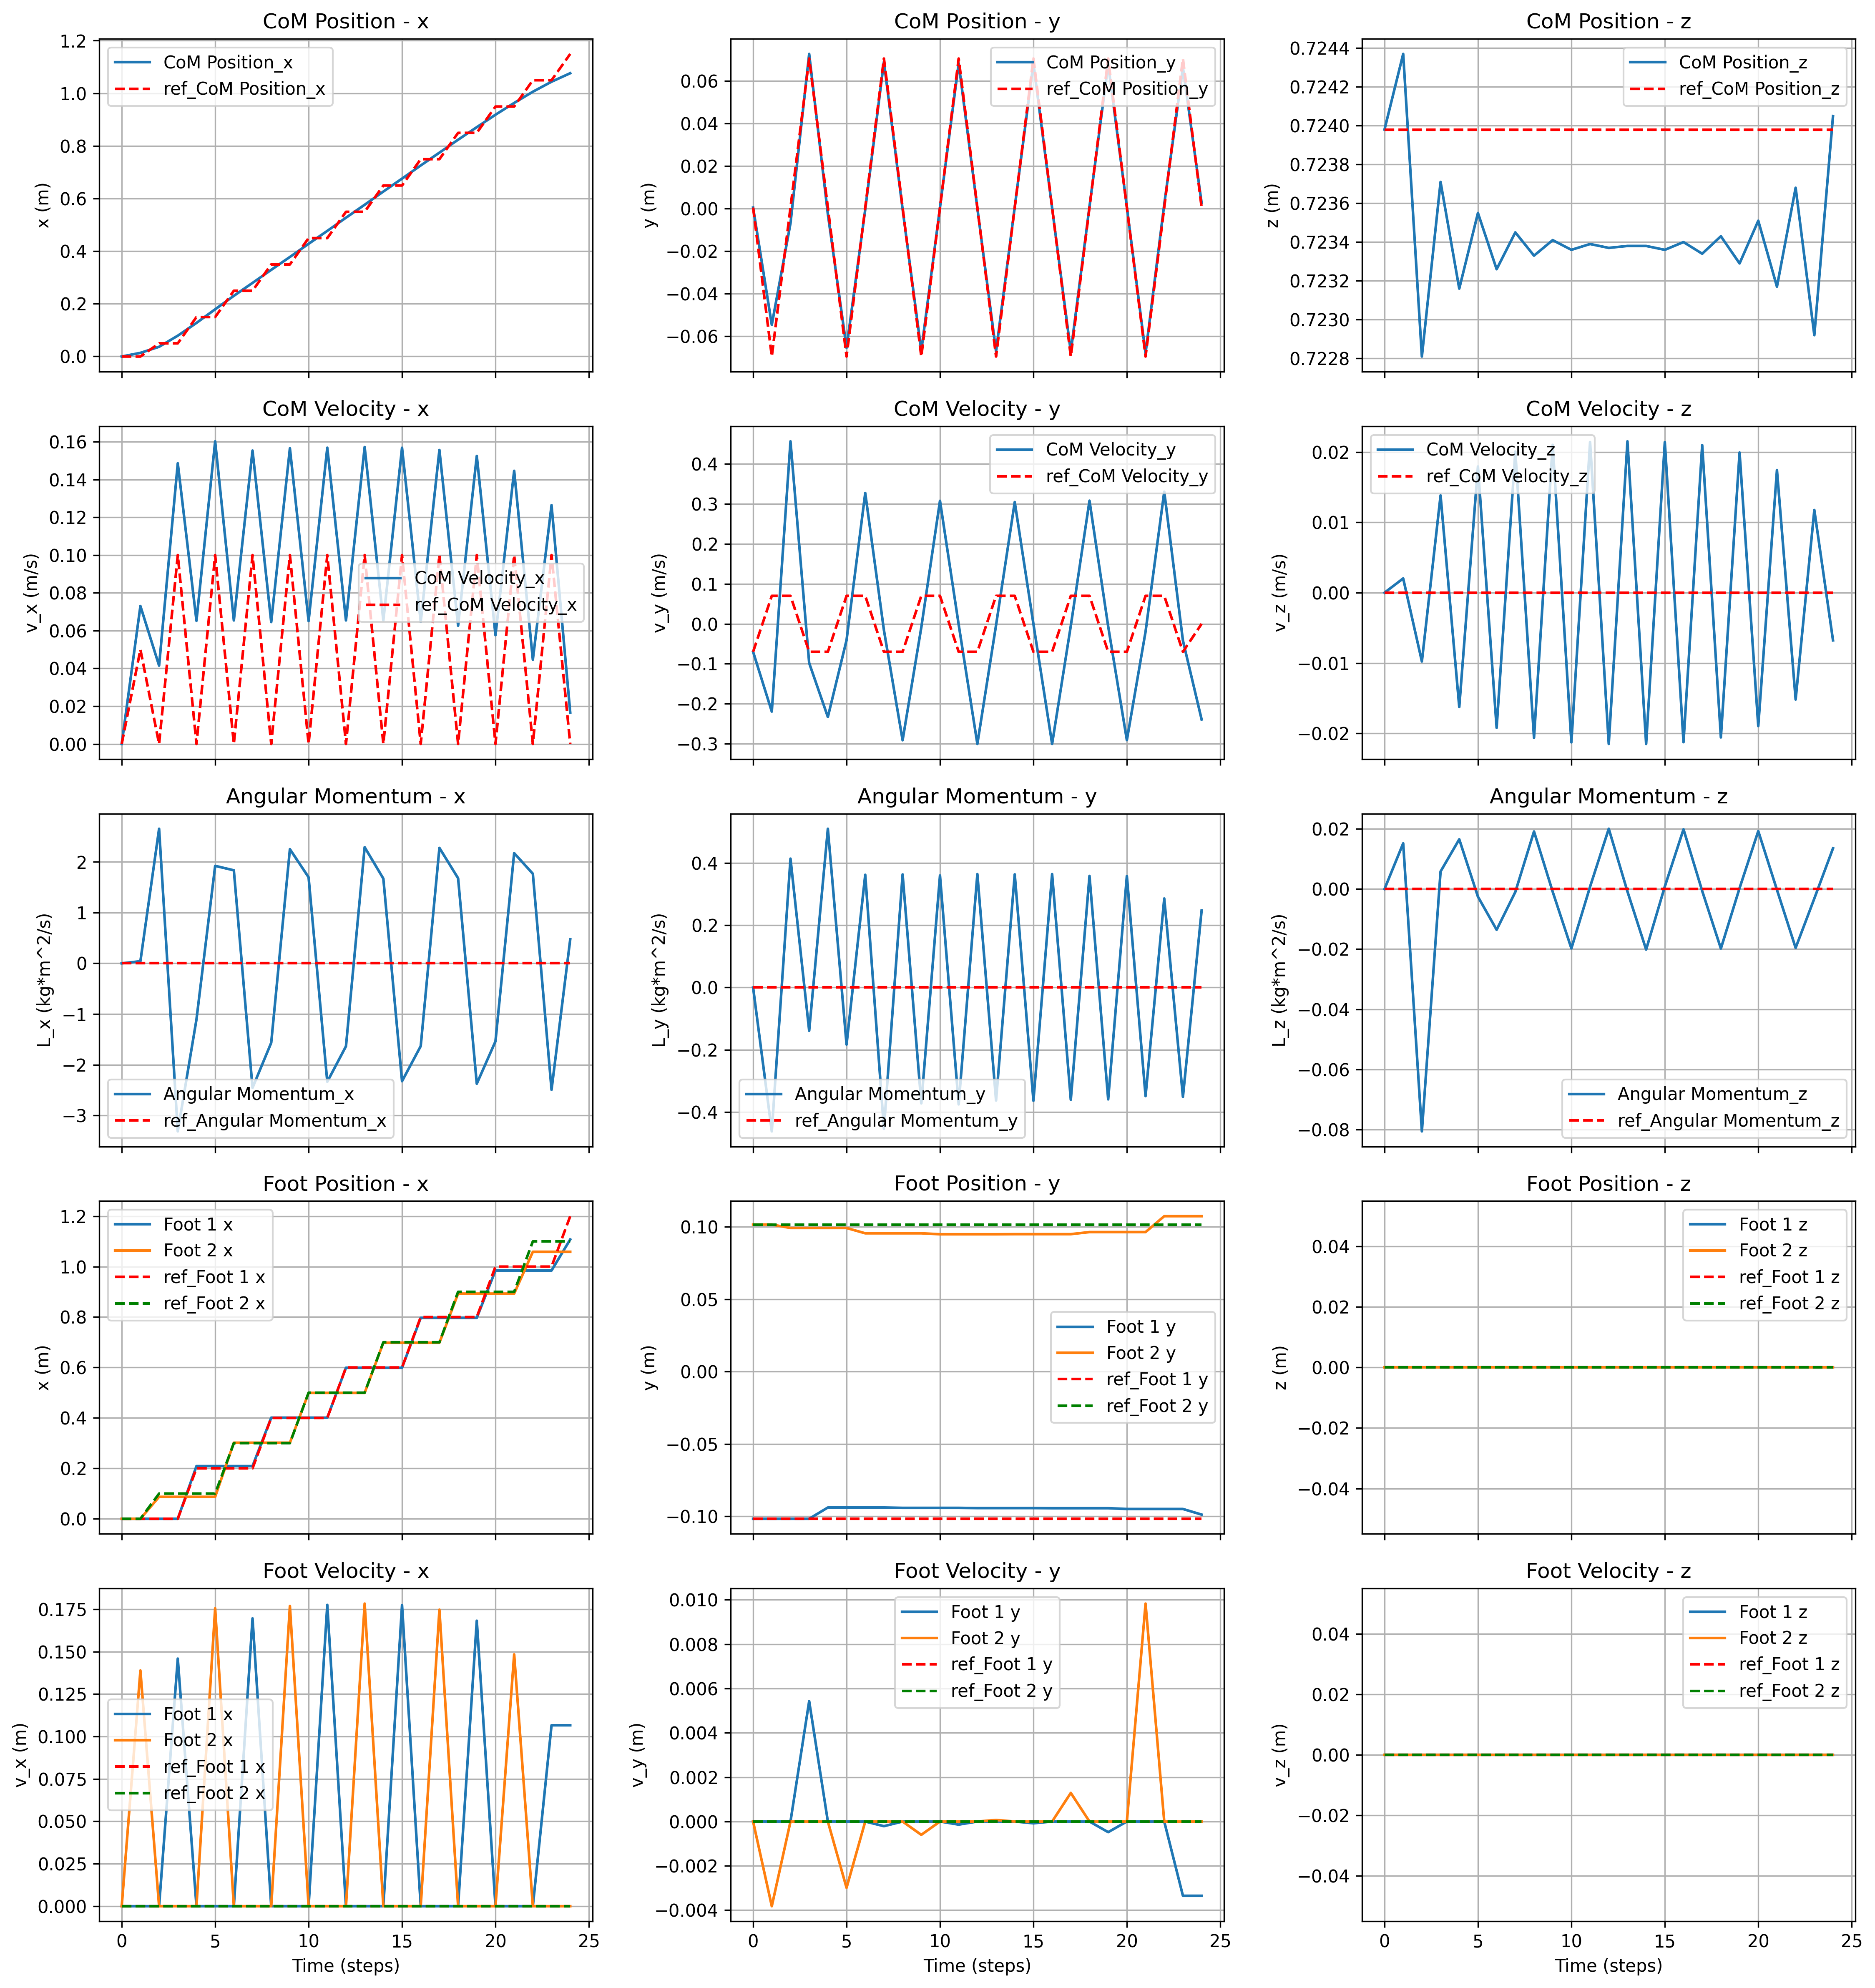
\includegraphics[width=0.8\textwidth]{figures/contact_x_walking.png}
    \caption{Trajectory vs Reference - Walking Task}
    \label{fig:yourlabel}
\end{figure}
\begin{table}[H]
    \centering
    \renewcommand{\arraystretch}{1.2}
    \resizebox{\textwidth}{!}{
        \begin{tabular}{c|c|c|c|c}
            \hline
            Interval & Right Foot (x,y,z) & Left Foot (x,y,z) & $\Sigma L_k$ & Sum Forces (x,y,z) \\
            \hline
            0 & (0.3186, 9.993, 49.064) & (0.3135, -8.822, 49.053) & (0, 0) & (0.6322, 1.1712, 98.1175) \\
            1 & (-2.9751, 12.258, 97.955) & (0, 0, 0) & (0, -1) & (-2.9751, 12.258, 97.9551) \\
            2 & (3.3303, -0.425, 48.897) & (-4.9023, -19.591, 49.650) & (0, 0) & (-1.5720, -20.016, 98.5473) \\
            3 & (0, 0, 0) & (-6.5058, 4.261, 97.490) & (-1, 0) & (-6.5058, 4.261, 97.4904) \\
            4 & (-7.0579, 14.053, 49.653) & (4.3045, -4.005, 49.156) & (0, 0) & (-2.7535, 10.048, 98.8092) \\
            5 & (-6.9692, 1.921, 97.308) & (0, 0, 0) & (0, -1) & (-6.9692, 1.921, 97.3081) \\
            6 & (3.0511, 1.817, 49.240) & (-5.6393, -16.023, 49.724) & (0, 0) & (-2.5882, -14.206, 98.9640) \\
            7 & (0, 0, 0) & (-6.7544, 0.511, 97.209) & (-1, 0) & (-6.7544, 0.511, 97.2091) \\
            8 & (-5.8989, 15.204, 49.739) & (3.3918, -2.610, 49.293) & (0, 0) & (-2.5070, 12.593, 99.0319) \\
            9 & (-6.8000, 0.593, 97.167) & (0, 0, 0) & (0, -1) & (-6.8000, 0.593, 97.1669) \\
            10 & (3.3444, 2.219, 49.301) & (-5.8685, -15.554, 49.761) & (0, 0) & (-2.5241, -13.335, 99.0619) \\
            11 & (0, 0, 0) & (-6.8143, -0.121, 97.149) & (-1, 0) & (-6.8143, -0.121, 97.1486) \\
            12 & (-5.9310, 15.393, 49.762) & (3.3932, -2.385, 49.310) & (0, 0) & (-2.5378, 13.008, 99.0720) \\
            13 & (-6.8282, 0.352, 97.144) & (0, 0, 0) & (0, -1) & (-6.8282, 0.352, 97.1443) \\
            14 & (3.3762, 2.297, 49.306) & (-5.9126, -15.492, 49.766) & (0, 0) & (-2.5364, -13.195, 99.0716) \\
            15 & (0, 0, 0) & (-6.8131, -0.182, 97.150) & (-1, 0) & (-6.8131, -0.182, 97.1495) \\
            16 & (-5.8724, 15.400, 49.756) & (3.3634, -2.397, 49.305) & (0, 0) & (-2.5091, 13.003, 99.0602) \\
            17 & (-6.7635, 0.425, 97.169) & (0, 0, 0) & (0, -1) & (-6.7635, 0.425, 97.1685) \\
            18 & (3.2848, 2.288, 49.282) & (-5.7111, -15.640, 49.747) & (0, 0) & (-2.4263, -13.351, 99.0282) \\
            19 & (0, 0, 0) & (-6.6265, 0.084, 97.216) & (-1, 0) & (-6.6265, 0.084, 97.2160) \\
            20 & (-5.4018, 15.280, 49.700) & (3.1738, -2.710, 49.254) & (0, 0) & (-2.2280, 12.571, 98.9543) \\
            21 & (-6.2994, 1.076, 97.326) & (0, 0, 0) & (0, -1) & (-6.2994, 1.076, 97.3264) \\
            22 & (2.6126, 2.308, 49.129) & (-4.3267, -16.682, 49.649) & (0, 0) & (-1.7142, -14.373, 98.7771) \\
            23 & (0, 0, 0) & (-5.5100, 1.696, 97.583) & (-1, 0) & (-5.5100, 1.696, 97.5828) \\
            \hline
        \end{tabular}
    }
    \caption{Summary of Forces and Foot Positions per Interval - Walking Task}
    \label{tab:data_table}
\end{table}
\begin{figure}[htbp]
    \centering
    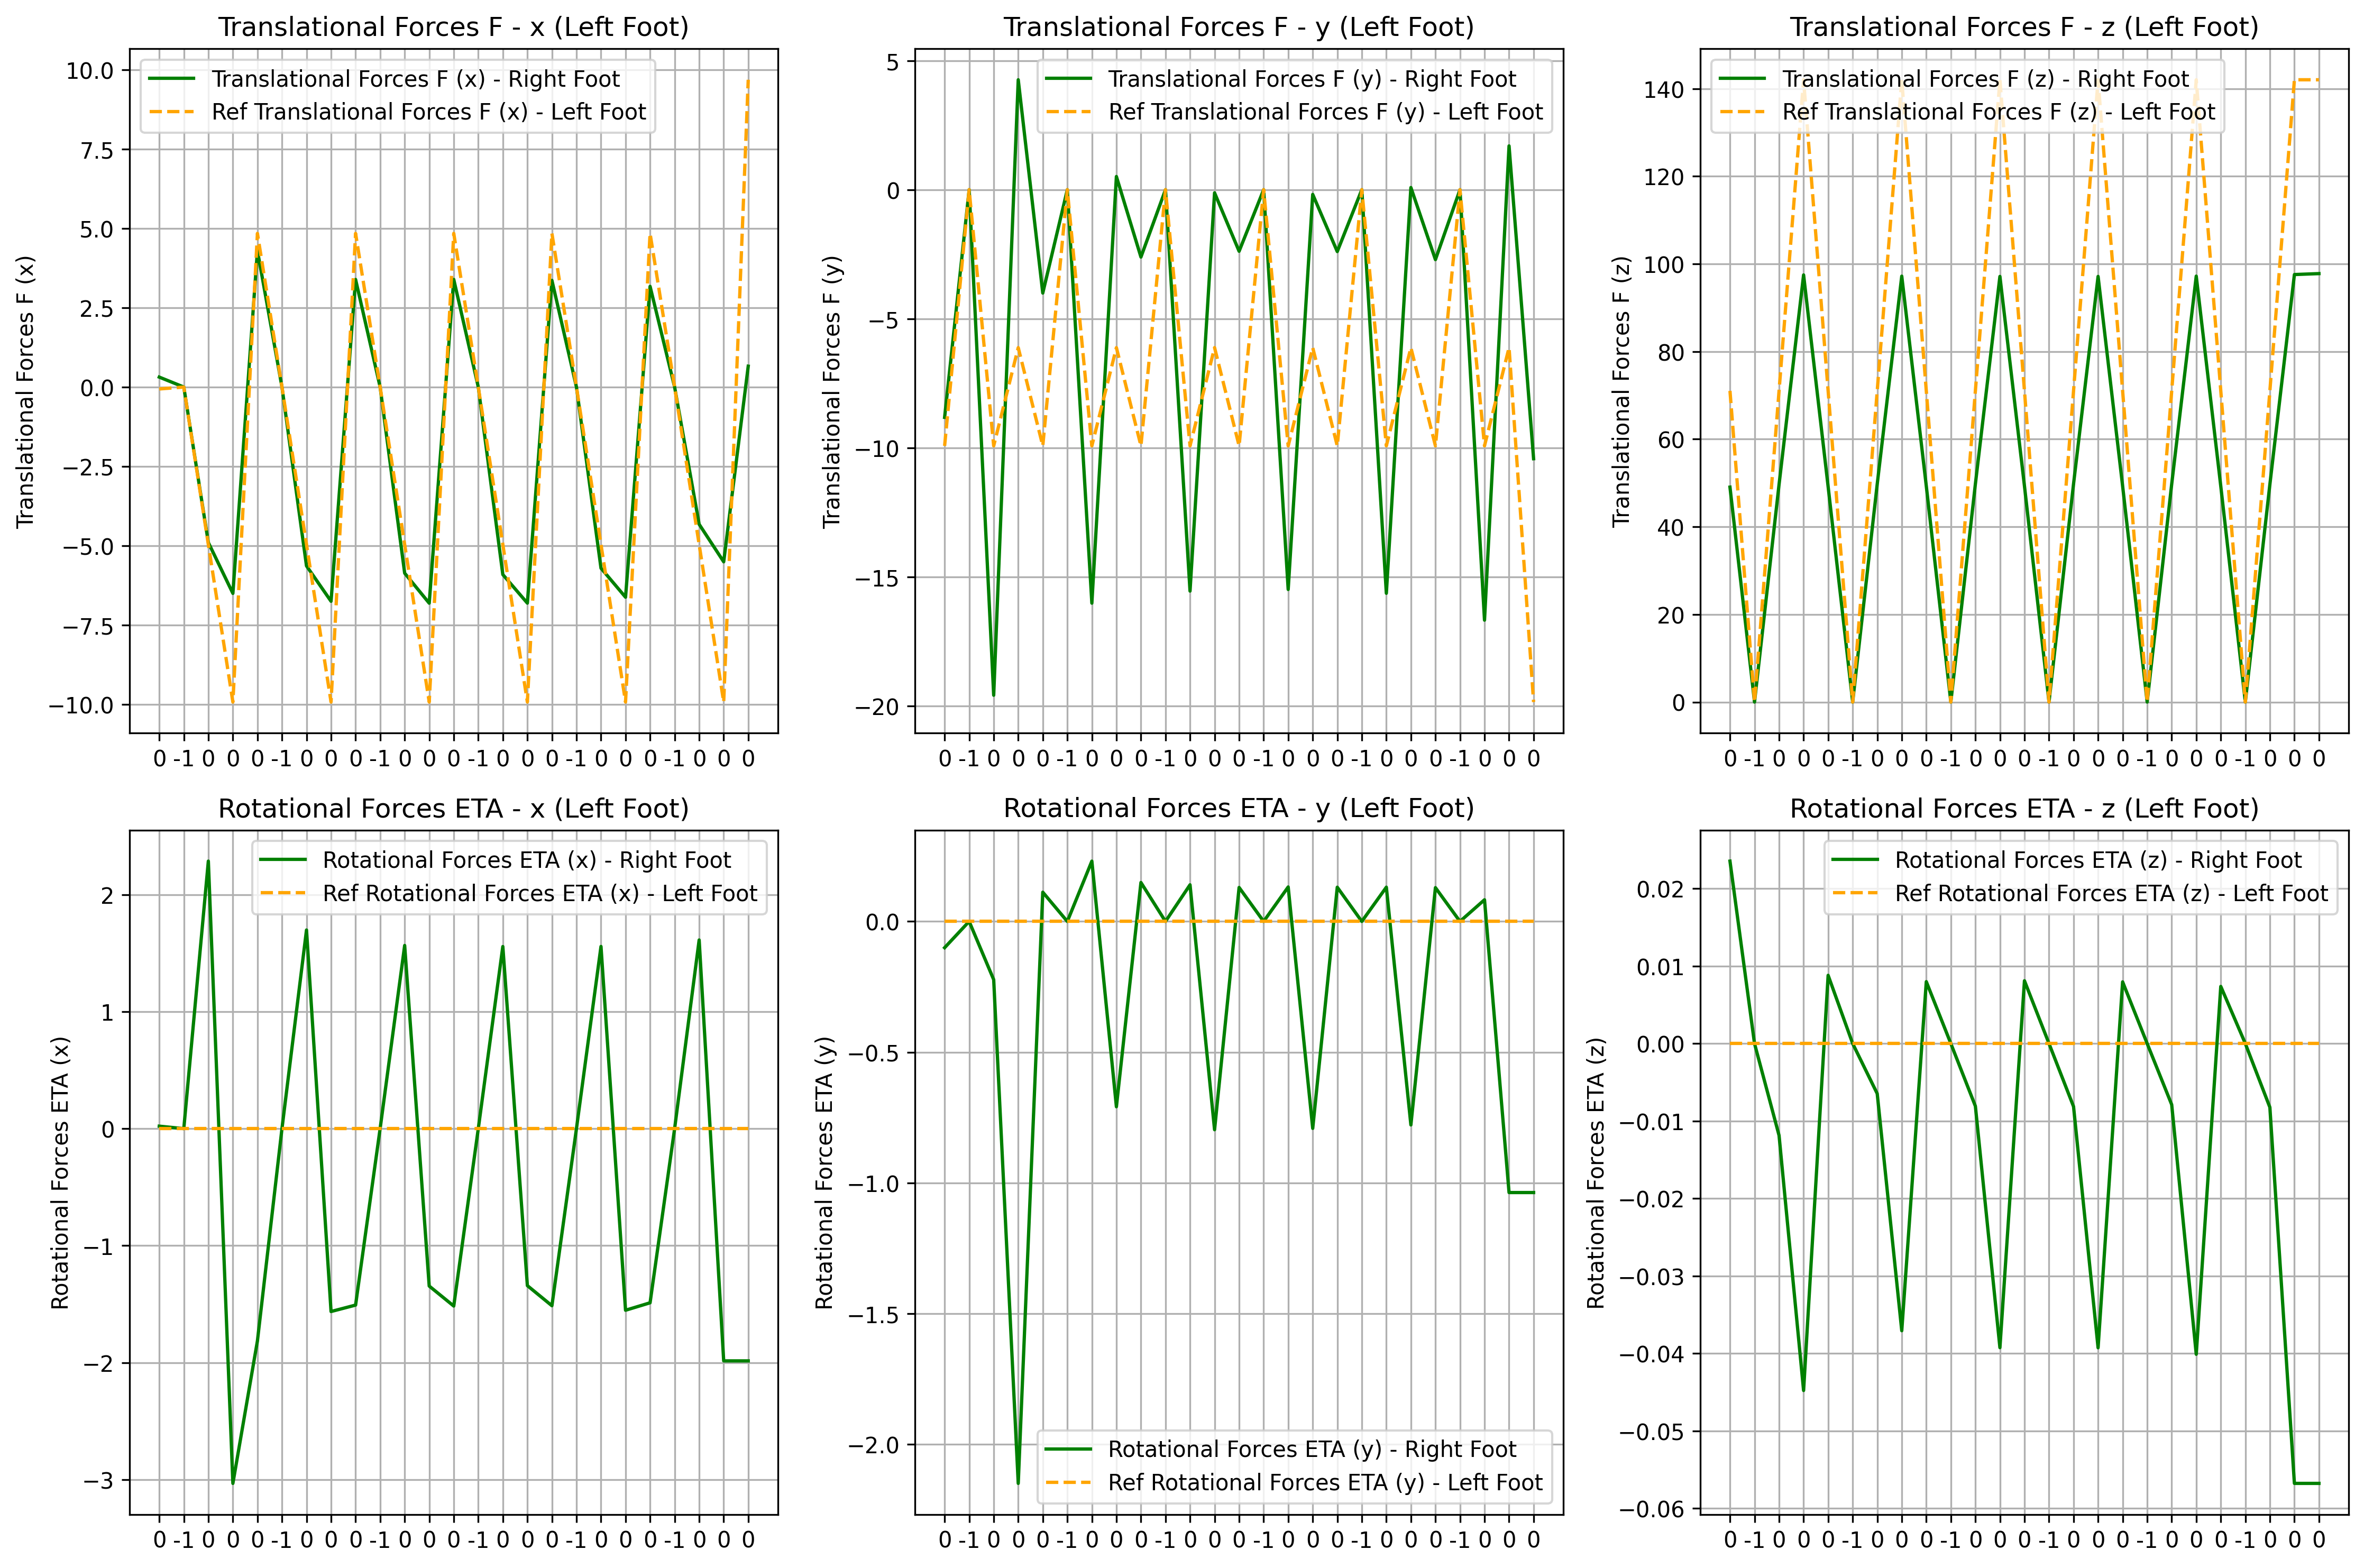
\includegraphics[width=0.8\textwidth]{figures/contact_forces_walking.png}
    \caption{Trajectory vs Reference Forces - Walking Task}
    \label{fig:contact_forces_walking}
\end{figure}


\paragraph{Simulation} 
Our work is built upon the repository available at [GitHub Link], which originally provides a comprehensive framework for simulating the HRP4 robot, including the dynamics model and control architecture. While the repository offers a complete baseline, we have extensively modified it by implementing our own dynamics and trajectory optimization framework. \\



\end{document}